\chapter{Channel Sharing Aided ISAC: An Energy-Efficient Sensing Scheduling Approach}
\label{chap2_twc1}

\section{Introduction} 
\label{chap2_sec_introduction}
With the rapid development of communication and sensing technologies, integrated sensing and communication (ISAC) networks have emerged as a promising paradigm for enabling advanced wireless services that require both high-throughput transmission and accurate environment sensing \cite{twc1.10012421,intro.9829746}. By utilizing the same spectrum resource for simultaneous data transmission and radar sensing, ISAC base stations can efficiently exploit valuable radio resources and enhance overall system performance. Consequently, ISAC is expected to play a vital role in future immersive services such as autonomous driving, digital twins, and augmented/virtual reality \cite{intro.9724245,intro.10049816}.

Although there have been several studies investigating the coordination between sensing and communication functions without incurring severe mutual interference, the stringent spectrum resources at radio access networks still lead to a crucial bottleneck in ISAC performance \cite{twc1.9665372,intro.10004900,intro.10663521}. To this end, this chapter proposes an approach to provide sensing services by actively reusing the channels of conventional cellular users, thereby effectively alleviating the scarcity of channel resources. Nevertheless, reusing cellular channels for sensing introduces a fundamental trade-off: it degrades the cellular users' quality of service (QoS), particularly in terms of throughput. This issue becomes exacerbated in multi-target sensing scenarios, where indiscriminately sensing multiple targets over a single user's channel may significantly impair that user's communication performance. Therefore, it is crucial to investigate an effective sensing scheduling mechanism, in which different sensing targets are strategically allocated to different cellular users' channels, with the objective of improving the overall sensing performance while strictly guaranteeing the QoS for cellular users.

To address these challenges, this chapter investigates an energy-efficient channel sharing aided ISAC framework, featuring a joint optimization of sensing scheduling and beamforming. The main contributions of this chapter are summarized as follows:

\begin{itemize}
	\item We propose an energy-efficient channel sharing aided ISAC with sensing scheduling, in which the ISAC base station (BS) performs sensing of multiple targets by reusing the channels of cellular users. We analyze the radar sensing echo signal when reusing the cellular user's channel, based on which we adopt the radar estimation information rate to quantify the sensing performance. We formulate a joint optimization of multi-target sensing scheduling, the BS's transmitting beamforming, and its receiving beamforming for each sensing target, with the objective of maximizing the energy efficiency for radar sensing while guaranteeing each cellular user's QoS.
	\item To address the non-convexity of the formulated optimization problem, we decompose it into two subproblems, including a beamforming vector optimization subproblem and a sensing scheduling optimization subproblem. For the beamforming vector optimization subproblem, we identify the property of its optimal solution and propose an efficient algorithm which is based on Dinkelbach's method and Lagrange duality to achieve the optimal beamforming (under a given sensing scheduling). For the sensing scheduling optimization subproblem under the given beamforming, we reformulate this subproblem as a matching game and solve it by using a swap matching based algorithm. We also prove the convergence of the swap matching based algorithm. We iteratively solve these two subproblems in an alternative manner to reach the solution of the original joint optimization problem.
	\item We demonstrate the performance advantage of our channel sharing aided ISAC in comparison with different benchmark schemes. Compared to several benchmark schemes, our algorithm can achieve better performance in terms of energy efficiency and the sum of radar estimation information rate. Moreover, compared with the solutions obtained by other existing algorithms/solvers, our proposed alternating algorithm can significantly reduce the computational time while guaranteeing the accuracy. 
\end{itemize}

The remainder of this chapter is organized as follows. We illustrate the system model and problem formulation in Section \ref{chap2_sec_systemmodel}. In Section \ref{sec:decomposition}, we decompose the original optimization problem into two subproblems and propose the corresponding algorithms for solving them. Section \ref{chap2_sec_result} demonstrates the performance of our channel sharing aided ISAC and Section \ref{chap2_sec_conclusion} summarizes this chapter.



\section{System Model of Channel Sharing-Aided ISAC} \label{chap2_sec_systemmodel}

\begin{figure*}[htbp]
    \centering
    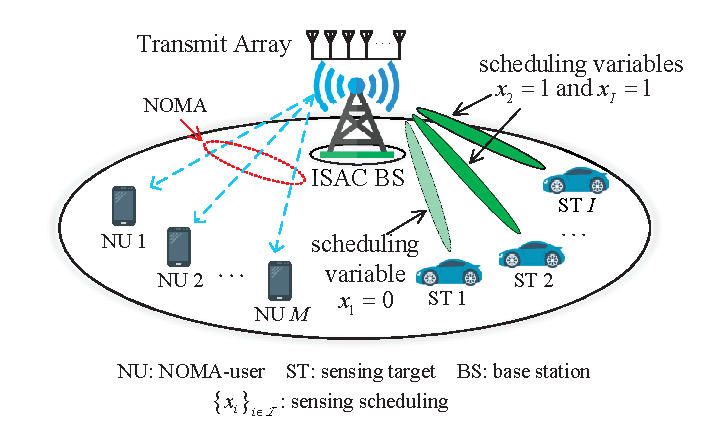
\includegraphics[width=0.9\textwidth]{figs_twc1_cld/Figure1.eps}
    \caption{An illustrative system model with 2 CUs and 5 STs}
    \label{chap2_fig_systemmodel}
\end{figure*}

Figure \ref{chap2_fig_systemmodel} illustrates the channel sharing aided ISAC in one cell coverage. Specifically, there exists one ISAC BS with $N_t$ transmit antennas and $N_r$ receive antennas, and $I$ single-antenna cellular users (CUs) denoted by $\mathcal{I}=\{1,2,...,I\}$. Each CU has a pre-assigned channel, and the channel of CU $i$ and the channel of CU $j$ ($\forall i,j\in\mathcal{I},i\neq j$) are orthogonal to each other, such that there is no co-channel interference between different CUs. To enable ISAC, the BS can reuse the CUs' channels to sense $N$ sensing targets (STs) denoted by $\mathcal{N}=\{1,2,...,N\}$, where each ST is allowed to be sensed over at most one CU's channel. We introduce a group of binary sensing scheduling variables $\{x_{ni}\}_{n\in\mathcal{N},i\in\mathcal{I}}$ as
\begin{align}
	x_{ni}=
	\begin{cases}
		1,&\text{CU $i$'s channel is reused for sensing ST $n$}, \\
		0,&\text{otherwise}.
	\end{cases}
\end{align}
Moreover, we introduce set $\mathcal{N}_i=\{n|x_{ni}=1,n\in\mathcal{N}\}\subseteq\mathcal{N}$ to denote the group of STs which are selected to be sensed over CU $i$'s channel, with $\mathcal{N}_i \cap \mathcal{N}_j=\emptyset$ ($\forall i,j\in\mathcal{I},i\neq j$).

\subsection{Modeling of Data Transmission}
With $\mathcal{N}_i$, the transmitted signal of the ISAC BS over CU $i$'s channel can be expressed as
\begin{equation}
	\mathbf{b}_i^{\text{BS}}=\mathbf{w}_is_i+\sum_{n\in\mathcal{N}_i}\mathbf{v}_nz_n,
	\label{transmit}
\end{equation}
where $\mathbf{w}_i\in\mathbb{C}^{N_t\times 1}$ denotes the BS's transmitting beamforming vector for CU $i$ and $s_i$ with $\mathbb{E}[|s_i|^2]=1$ denotes the information symbol for CU $i$. Meanwhile, in eq. (2), $\mathbf{v}_n\in\mathbb{C}^{N_t\times 1}$ denotes the BS's transmitting beamforming vector for ST $n$, and $z_n$ with $\mathbb{E}[|z_n|^2]=1$ denotes the symbol of the dedicated sensing signal for ST $n$.
Therefore, the received signal at CU $i$ can be expressed as
\begin{equation}
	y_i^{\text{CU}}=\mathbf{h}_i^H\mathbf{b}_i^{\text{BS}}+n_C=\mathbf{h}_i^H\mathbf{w}_is_i+\mathbf{h}_i^H\sum_{n\in\mathcal{N}_i}\mathbf{v}_nz_n+n_C,
	\label{CU_receive}
\end{equation}
where $\mathbf{h}_i\in\mathbb{C}^{N_t\times 1}$ denotes the channel gain between the ISAC BS and CU $i$, and $n_C$ denotes the circularly symmetric complex Gaussian noise with variance $\sigma_C^2$. Correspondingly, the throughput achieved by CU $i$ can be expressed as 
\begin{equation}
	R_i^{\text{com}}=B_i\log_2\left(1+\frac{|\mathbf{h}_i^H\mathbf{w}_i|^2}{\sum_{n\in\mathcal{N}_i}|\mathbf{h}_i^H\mathbf{v}_n|^2+\sigma_C^2}\right),
	\label{CU_R}
\end{equation}
where $B_i$ denotes the channel bandwidth of CU $i$. In this work, we consider that the BS's transmitting beamforming vectors for the CUs, i.e., $\{\mathbf{w}_i\}_{i\in\mathcal{I}}$, are fixed. We aim at guaranteeing each CU's throughput requirement by properly controlling the sensing scheduling and the BS's transmitting beamforming for sensing, i.e., constraint (2.10) in our problem formulation in Section 2.2.3.
	
\subsection{Modeling of Sensing}
We assume that ST $n$'s azimuth $\theta_n$ is known by the ISAC BS. As a result, the received signal at the ISAC BS over CU $i$'s channel can be expressed as
\begin{equation}
	\mathbf{y}_{i}^{\text{BS}}=\sum_{n\in\mathcal{N}_i}\alpha_{ni}\mathbf{A}(\theta_n)\mathbf{b}_i^{\text{BS}}+\mathbf{n}_S,
	\label{BS_receive}
\end{equation}
where $\mathbf{A}(\theta_n)\triangleq\mathbf{a}_r(\theta_n)\mathbf{a}_t^H(\theta_n)\in\mathbb{C}^{N_r\times N_t}$. $\alpha_{ni}$ is the complex channel between ST $n$ and the ISAC BS over CU $i$'s channel, and $\mathbf{n}_S$ is the circularly symmetric complex Gaussian noise with variance $\sigma_S^2$ of each element. The dependencies of the transmitting steering vector $\mathbf{a}_t(\theta_n)$ and the receiving steering vector $\mathbf{a}_r(\theta_n)$ on angle $\theta_n$ can be respectively expressed as 
\begin{equation}
	\mathbf{a}_t(\theta_n)=\frac{1}{\sqrt{N_t}}\left[1,e^{-j2\pi d_t\sin\theta_n},...,e^{-j2\pi d_t(N_t-1)\sin\theta_n}\right]^T,
\end{equation}
\begin{equation}
	\mathbf{a}_r(\theta_n)=\frac{1}{\sqrt{N_r}}\left[1,e^{-j2\pi d_r\sin\theta_n},...,e^{-j2\pi d_r(N_r-1)\sin\theta_n}\right]^T,
\end{equation}
where $d_t$ denotes the spacing of transmitting antenna array normalized by the wavelength, and $d_r$ denotes the spacing of receiving antenna array normalized by the wavelength.
	
At the ISAC BS, different echoes from the STs can be obtained via the receiver filtering by multiplying the BS's receiving beamforming vector. Specifically, we use $\mathbf{u}_n\in\mathbb{C}^{N_r\times 1}$ to denote the BS's receiving beamforming vector for ST $n$. Thus, the echo from ST $n$ over CU $i$'s channel after the receiver filtering can be expressed as $x_{ni}\mathbf{u}_n^H\mathbf{y}_{i}^{\text{BS}}$.
Correspondingly, the radar sensing performance for sensing ST $n$ over CU $i$'s channel is characterized by the radar estimation information rate (REIR) as
\begin{equation}
	R_{ni}^{\text{rad}}=\frac{\delta}{2T}\log_2\left(1+2TB_i\frac{x_{ni}|\alpha_{ni}|^2|\mathbf{u}_n^H\mathbf{A}(\theta_n)\mathbf{v}_n|^2}{\mathbf{u}_n^H\mathbf{\Gamma}_{ni}\mathbf{u}_n}\right),
	\label{REIR}
\end{equation}
where $\delta$ denotes the radar duty factor, and $T$ denotes the radar pulse duration. In eq. (\ref{REIR}), $\mathbf{\Gamma}_{ni}$ denotes the total interference for sensing ST $n$ over CU $i$'s channel, and it can be shown as
\begin{equation}
\begin{split}
	\mathbf{\Gamma}_{ni}=& \mathop{\underbrace{\sum_{p\in\mathcal{N}_i}\alpha_{pi}^2\mathbf{A}(\theta_p)\mathbf{w}_i\mathbf{w}_i^H\mathbf{A}^H(\theta_p)}\limits_{\text{Interference from the communication signal}}}+\mathop{\underbrace{x_{ni}\alpha_{ni}^2\mathbf{A}(\theta_n)\left(\sum_{q\in\mathcal{N}_i, q\neq n}\mathbf{v}_q\mathbf{v}_q^H\right)\mathbf{A}^H(\theta_n)}\limits_{\text{Interference from other sensing signals on ST $n$'s echo}}}\\&+\mathop{\underbrace{\sum_{p\in\mathcal{N}_i ,p\neq n}\alpha_{pi}^2\mathbf{A}(\theta_p)\left(\sum_{q\in\mathcal{N}_i}\mathbf{v}_q\mathbf{v}_q^H\right)\mathbf{A}^H(\theta_p)}\limits_{\text{Interference from other STs' echoes}}}+\mathop{\underbrace{\sigma_S^2\mathbf{I}}\limits_{\text{Noise}}}.
	\label{Gamma}
\end{split}
\end{equation}
It can be observed from eq. (\ref{REIR}) that $R_{ni}^{\text{rad}}=0$ if ST $n$ is not sensed over CU $i$'s channel (i.e., $x_{ni}=0$). Thus, the total REIR of ST $n$ can be expressed as $\sum_{i\in\mathcal{I}}R_{ni}^{\text{rad}}$. 

\subsection{Problem Formulation}
	
In this chapter, we aim at maximizing the energy efficiency (MEE) for radar sensing which is denoted by the ratio of the total STs' REIR overall the total power consumption, while guaranteeing each CU's throughput requirement. To achieve this goal, we formulate a joint optimization of sensing scheduling variables $\{x_{ni}\}_{n\in\mathcal{N},i\in\mathcal{I}}$, the BS's transmitting beamforming vectors $\{\mathbf{v}_n\}_{n\in\mathcal{N}}$ for sensing the STs, and its receiving beamforming vectors $\{\mathbf{u}_n\}_{n\in\mathcal{N}}$ for filtering the STs' echoes as follows.
\begin{flalign}
	\text{(MEE):~}
	&\max  \frac{\sum_{n\in\mathcal{N}}\sum_{i\in\mathcal{I}}R^{\text{rad}}_{ni}}{\mathbf{Tr}\left(\sum_{i\in\mathcal{I}}\mathbf{w}_i\mathbf{w}_i^H+\sum_{n\in\mathcal{N}}\mathbf{v}_n\mathbf{v}_n^H\right)+P^C}\nonumber\\
	\text{subject to:~}
	&R_i^{\text{com}}\ge R_i^{\text{req}},\forall i\in\mathcal{I}, \label{comm}
	\\
	&\sum_{i\in\mathcal{I}}x_{ni}\le 1, \forall n\in\mathcal{N}, \label{eachn}
	\\
	&\sum_{n\in\mathcal{N}}x_{ni}\le J_i^{\text{max}}, \forall i\in\mathcal{I}, \label{eachi}
	\\
	&x_{ni}\in\{0,1\}, \forall n\in\mathcal{N}, \forall i\in\mathcal{I}, \label{x_ni}
	\\
	\text{variables:~} & {\{x_{ni}\}_{n\in\mathcal{N},i\in\mathcal{I}}}, {\{\mathbf{v}_n\}_{n\in\mathcal{N}}}, \text{~and~} {\{\mathbf{u}_n\}_{n\in\mathcal{N}}}.\nonumber
\end{flalign}
In the objective function, $\mathbf{Tr}\left(\sum_{i\in\mathcal{I}}\mathbf{w}_i\mathbf{w}_i^H+\sum_{n\in\mathcal{N}}\mathbf{v}_n\mathbf{v}_n^H\right)$ denotes the total transmitting power of the ISAC BS and $\mathbf{Tr}(\cdot)$ denotes the trace function. Parameter $P^C$ denotes the circuit power consumption which is a constant. Constraint (\ref{comm}) ensures that each CU $i$ can achieve its required throughput denoted by $R_i^{\text{req}}$. Constraint (\ref{eachn}) ensures that at most one CU's channel is reused for sensing ST $n$. Constraint (\ref{eachi}) indicates that at most $J_i^{\text{max}}$ STs can be sensed over CU $i$'s channel.

\section{Proposed Algorithms for Solving Problem (MEE)}
\label{sec:decomposition}
	
Problem (MEE) is a mixed binary nonlinear programming problem. The binary sensing scheduling $\{x_{ni}\}_{n\in\mathcal{N},i\in\mathcal{I}}$ and the BS's  beamforming vectors $\{\mathbf{v}_n\}_{n\in\mathcal{N}}$ and $\{\mathbf{u}_n\}_{n\in\mathcal{N}}$ are tightly coupled in the objective function. Moreover, the fractional structure of the objective function leads to a non-convex optimization problem. Therefore, it is challenging to solve Problem (MEE) directly. To address this difficulty, we propose a framework of alternating optimization to obtain the solution to Problem (MEE). The details are as follows.
	
\subsection{Decomposition of Problem (MEE)}
	
To address the difficulty due to the mixed binary and non-convexity, we decompose Problem (MEE) into two subproblems, including Problem (MEE-BVO) to optimize the continuous beamforming vectors and Problem (MEE-SSO) to optimize the binary sensing scheduling variables.
	
\subsubsection{Beamforming vectors optimization (BVO) under the given sensing scheduling}
Given the sensing scheduling $\{x_{ni}\}_{n\in\mathcal{N},i\in\mathcal{I}}$, Problem (MEE) turns into the following Problem (MEE-BVO).
\begin{flalign}
	\text{(MEE-BVO):~}
	&\max  \frac{\sum_{n\in\mathcal{N}}\sum_{i\in\mathcal{I}}R^{\text{rad}}_{ni}}{\mathbf{Tr}\left(\sum_{i\in\mathcal{I}}\mathbf{w}_i\mathbf{w}_i^H+\sum_{n\in\mathcal{N}}\mathbf{v}_n\mathbf{v}_n^H\right)+P^C}\nonumber\\
	\text{subject to:~}
	&\text{constraint~} (\ref{comm}),\nonumber
	\\
	\text{variables:~} & {\{\mathbf{v}_n\}_{n\in\mathcal{N}}} \text{~and~} {\{\mathbf{u}_n\}_{n\in\mathcal{N}}}.\nonumber
\end{flalign}

\subsubsection{Sensing scheduling optimization (SSO) under the given beamforming vectors}
Given the beamforming vectors $\{\mathbf{v}_n\}_{n\in\mathcal{N}}$ and $\{\mathbf{u}_n\}_{n\in\mathcal{N}}$, after performing some mathematical manipulations, Problem (MEE-SSO) for optimizing the sensing scheduling can be expressed as follows.
\begin{flalign}
	\text{(MEE-SSO):~}
	&\max  \Lambda(\{x_{ni}\}_{n\in\mathcal{N},i\in\mathcal{I}})=\sum_{n\in\mathcal{N}}\sum_{i\in\mathcal{I}}R^{\text{rad}}_{ni}\nonumber\\
	\text{subject to:~}
	&\text{constraints~} (\ref{comm}), (\ref{eachn}), (\ref{eachi}) \text{~and~} (\ref{x_ni}),\nonumber
	\\
	\text{variables:~} & {\{x_{ni}\}_{n\in\mathcal{N},i\in\mathcal{I}}}.\nonumber
\end{flalign}
	
\begin{figure*}
	\centering
	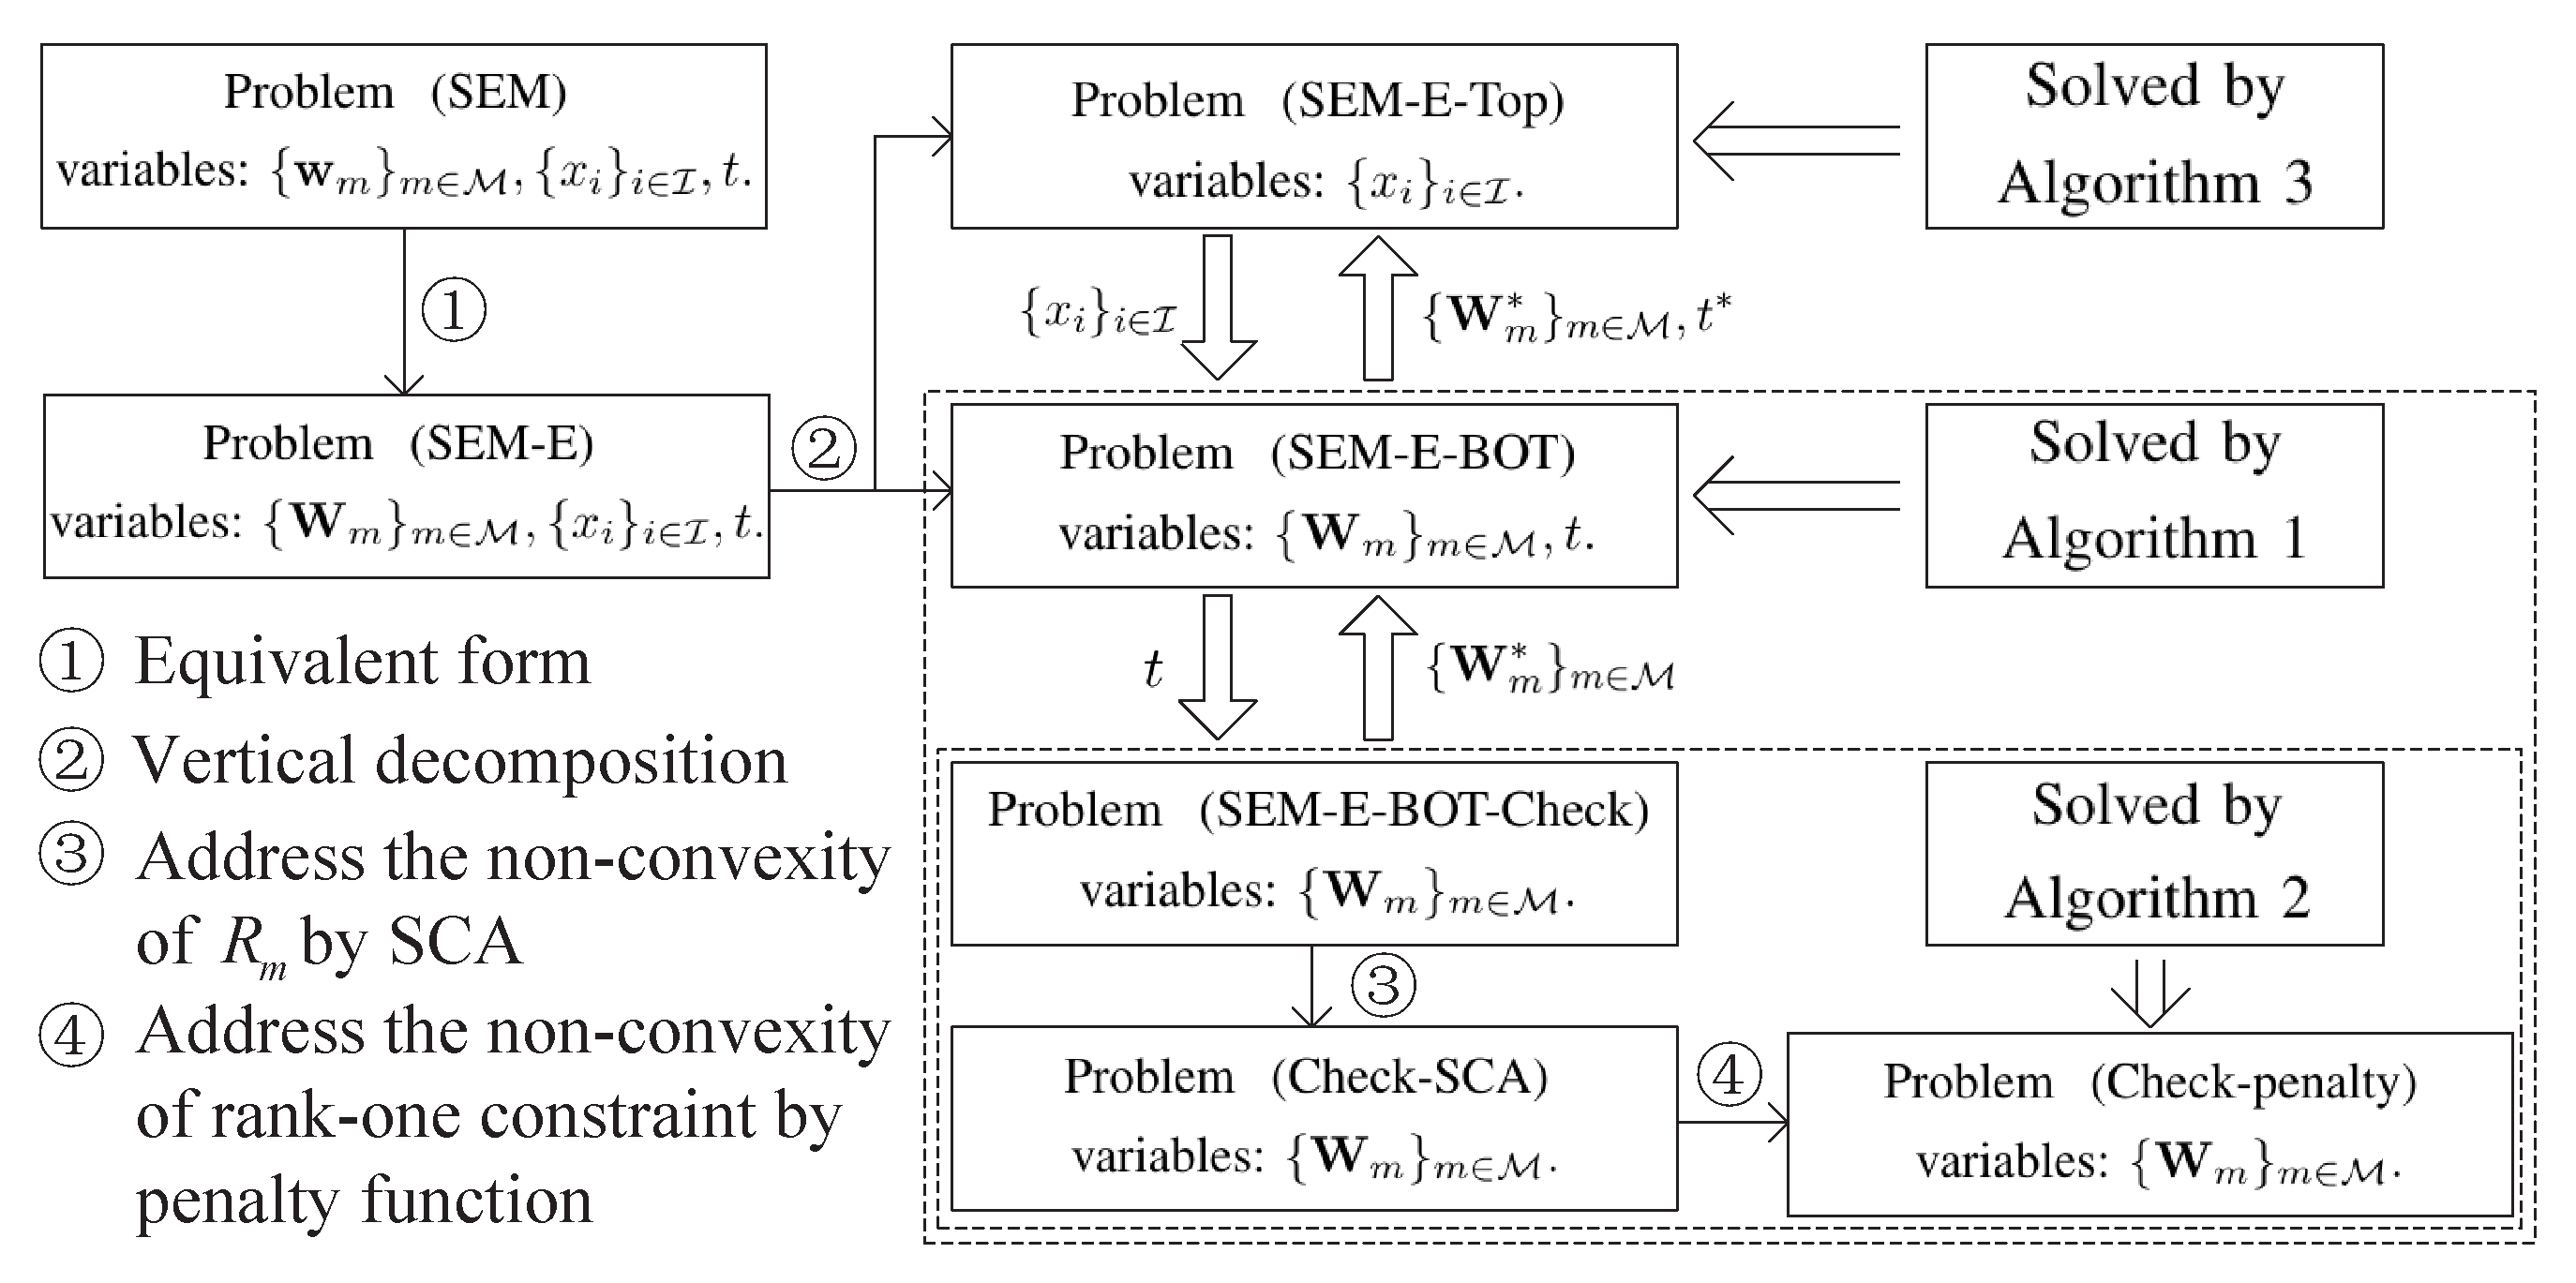
\includegraphics[width=0.9\textwidth]{figs_twc1_cld/Figure2.eps}
	\caption{Decomposition of Problem (MEE) into two subproblems}
	\label{decompose}
\end{figure*}

As shown in Figure \ref{decompose}, Problem (MEE-BVO) and Problem (MEE-SSO) are executed in an alternative manner to solve the original Problem (MEE). 
It is different from existing algorithms which use the block coordinate descent and successive convex approximation to obtain the solution after relaxing the binary variables. 
In the remainder of this section, we first perform an equivalent transformation for the fractional structure of Problem (MEE-BVO) by leveraging Dinkelbach's method. 
Then, we use Lagrange duality to derive the underlying structure of the optimal solutions by identifying its convexity.
In particular, we formulate Problem (MEE-SSO) as a many-to-one matching problem and propose the corresponding algorithm to obtain the optimal sensing scheduling.
	
\subsection{Proposed Algorithm for Solving Problem (MEE-BVO)}
	
Problem (MEE-BVO) is a strictly non-convex problem due to its fractional structure, which is challenging to solve. To tackle with its non-convexity, we first leverage the Dinkelbach's method to deal with the objective function of Problem (MEE-BVO). For the sake of clear presentation, we define
\begin{equation}
	f_1^{\text{obj}}\triangleq\sum_{n\in\mathcal{N}}\sum_{i\in\mathcal{I}}R_{ni}^{\text{rad}},\label{f1}
\end{equation}
and 
\begin{equation}
f_2^{\text{obj}}\triangleq \mathbf{Tr}\left(\sum_{i\in\mathcal{I}}\mathbf{w}_i\mathbf{w}_i^H+\sum_{n\in\mathcal{N}}\mathbf{v}_n\mathbf{v}_n^H\right)+P^C.\label{f2}
\end{equation} 
By introducing an auxiliary variable $\mu$ as 
\begin{equation}
	\mu\le \frac{f_1^{\text{obj}}}{f_2^{\text{obj}}},\label{mu}
\end{equation}
we can transform Problem (MEE-BVO) into the following equivalent form.
\begin{flalign}
	\text{(BVO-E):~}
	&\max~  \mu\nonumber\\
	\text{subject to:~}
	&\text{constraint~} (\ref{comm}),\nonumber
	\\
	&f_1^{\text{obj}}-\mu f_2^{\text{obj}}\ge 0,\label{mu_tran}
	\\
	\text{variables:~} & {\mu}, {\{\mathbf{v}_n\}_{n\in\mathcal{N}}} \text{~and~} {\{\mathbf{u}_n\}_{n\in\mathcal{N}}}.\nonumber
\end{flalign}
For Problem (BVO-E), we observe that for a given value of $\mu$, the optimization problem is feasible if $f_1^{\text{obj}}-\mu f_2^{\text{obj}}\ge 0$. In particular, Problem (MEE-BVO) achieves the optimal solutions if and only if Problem (BVO-E) achieves the optimal solutions with the optimal $\mu^*$. Moreover, $f_1^{\text{obj}}-\mu f_2^{\text{obj}}$ is strictly decreasing in $\mu$, which indicates that the optimal value $\mu^*$ is obtained when constraint (\ref{mu_tran}) is strictly binding. Therefore, to solve Problem (BVO-E), for a given value of $\mu$, we solve the following subproblem
\begin{flalign}
	\text{(BVO-E-Sub):~}
	&\max~  \sum_{n\in\mathcal{N}}\sum_{i\in\mathcal{I}}R^{\text{rad}}_{ni}\nonumber-\mu\left(\mathbf{Tr}\left(\sum_{i\in\mathcal{I}}\mathbf{w}_i\mathbf{w}_i^H+\sum_{n\in\mathcal{N}}\mathbf{v}_n\mathbf{v}_n^H\right)+P^C\right)\nonumber\\
	\text{subject to:~}
	&\text{constraint~} (\ref{comm}),\nonumber
	\\
	\text{variables:~} & {\{\mathbf{v}_n\}_{n\in\mathcal{N}}} \text{~and~} {\{\mathbf{u}_n\}_{n\in\mathcal{N}}}.\nonumber
\end{flalign}
After solving Problem (BVO-E-Sub) and obtaining the corresponding optimal values $\{f_1^{\text{obj},*},f_2^{\text{obj},*}\}$ of $\{f_1^{\text{obj}},f_2^{\text{obj}}\}$ under the current value of $\mu$ (i.e., Step 12 of Algorithm 1), we can further update the value of $\mu$ as
\begin{equation}
	\mu= \frac{f_1^{\text{obj},*}}{f_2^{\text{obj},*}}.\label{update}
\end{equation}
It can be proved that the convergence is guaranteed by iteratively updating $\mu$ according to eq. (\ref{update}) since $\mu$ is non-decreasing after each iteration \cite{twc1.schaible1983fractional}. These iterative operations continue until $|f_1^{\text{obj},*}-\mu f_2^{\text{obj},*}|$ is no greater than a given threshold (i.e., Step 13 of Algorithm 1).
	
For a given value of $\mu$, we then solve Problem (BVO-E-Sub). To solve Problem (BVO-E-Sub), we firstly identify the following feature. 
\begin{proposition}
	\label{proposition1}
	In Problem (BVO-E-Sub), the optimal receiving beamforming vectors that maximize the radar sensing REIR can be given as
	\begin{equation}
		\mathbf{u}_n^*=\max\limits_{i\in\mathcal{I}}\left\{\frac{x_{ni}\mathbf{\Gamma}_{ni}^{-1}\mathbf{A}(\theta_n)\mathbf{v}_n}{\mathbf{v}_n^H\mathbf{A}^H(\theta_n)\mathbf{\Gamma}_{ni}^{-1}\mathbf{A}(\theta_n)\mathbf{v}_n}\right\}.
		\label{u^*}
	\end{equation}
\end{proposition}
\begin{proof}
	According to the minimum variance distortionless response (MVDR) problem \cite{twc1.van2002optimum}, for each ST $n$, the design of $\mathbf{u}_n$ can be expressed as
\begin{equation}
	\max_{\mathbf{u}_n}~ \zeta_{ni}^{\text{echo}}= \frac{x_{ni}|\alpha_{ni}|^2|\mathbf{u}_n^H\mathbf{A}(\theta_n)\mathbf{v}_n|^2}{\mathbf{u}_n^H\mathbf{\Gamma}_{ni}\mathbf{u}_n}.
\end{equation}
Let $\frac{\partial\zeta_{ni}^{\text{echo}}}{\partial\mathbf{u}_n}=0$, we can derive that
\begin{align}
	\mathbf{u}_n=
	\begin{cases}
		\frac{\mathbf{\Gamma}_{ni}^{-1}\mathbf{A}(\theta_n)\mathbf{v}_n}{\mathbf{v}_n^H\mathbf{A}^H(\theta_n)\mathbf{\Gamma}_{ni}^{-1}\mathbf{A}(\theta_n)\mathbf{v}_n},&\text{when~} x_{ni}=1,\\
		0,&\text{otherwise}.
	\end{cases}
\end{align}
Therefore, the optimal receiving beamforming vector that maximizes the radar sensing REIR can be given as eq. (\ref{u^*}).
\end{proof}
	
Substituting eq. (\ref{u^*}) into eq. (\ref{REIR}), the REIR for sensing ST $n$ over CU $i$'s channel can be calculated as
\begin{equation}
		R_{ni}^{\text{rad}}=\frac{\delta}{2T}\log_2\left(1+2TB_ix_{ni}\mathbf{v}_n^H\mathbf{\Phi}_{ni}\mathbf{v}_n\right),
	\label{REIR_new}
\end{equation}
where $\mathbf{\Phi}_{ni}=|\alpha_{ni}|^2\mathbf{A}^H(\theta_n)\mathbf{\Gamma}_{ni}^{-1}\mathbf{A}(\theta_n)$.
	
	
	
For each ST $n$, we define $\mathbf{V}_n\triangleq\mathbf{v}_n\mathbf{v}_n^H$, with three constraints $\mathbf{V}_n\succeq 0$, $\mathbf{V}_n=\mathbf{V}_n^H$, and rank($\mathbf{V}_n$) = 1. For CU $i$, we define $\mathbf{H}_i\triangleq\mathbf{h}_i\mathbf{h}_i^H$ and $\mathbf{W}_i\triangleq\mathbf{w}_i\mathbf{w}_i^H$.
Then, with eq. (\ref{CU_R}), constraint (\ref{comm}) can be rewritten as
\begin{equation}
	\sum_{n\in\mathcal{N}_i}\mathbf{Tr}\left(\mathbf{H}_i\mathbf{V}_n\right)\le \epsilon_i,\forall i\in\mathcal{I},\label{comm-re}
\end{equation}
where $\epsilon_i$ can be expressed as
\begin{equation}
	\epsilon_i=\frac{\mathbf{Tr}\left(\mathbf{H}_i\mathbf{W}_i\right)-\sigma_C^2\left(2^{\frac{R_i^{\text{req}}}{B_i}}-1\right)}{2^{\frac{R_i^{\text{req}}}{B_i}}-1}.\label{epsilon}
\end{equation}
We first address the non-convexity of $\mathbf{\Phi}_{ni}$ by using an iterative approach in which we set the values of $\{\mathbf{V}_n\}_{n\in\mathcal{N}}$ in $\mathbf{\Phi}_{ni}$ at each iteration according to the optimal values of $\{\mathbf{V}_n\}_{n\in\mathcal{N}}$ obtained in the previous iteration. Specifically, we calculate
\begin{equation}
	\mathbf{\Phi}_{ni}^{\prime}=|\alpha_{ni}|^2\mathbf{A}^H(\theta_n)\mathbf{\Gamma}_{ni}^{-1}(\{\mathbf{V}_n^\prime\}_{n\in\mathcal{N}})\mathbf{A}(\theta_n),
	\label{SCA}
\end{equation}
where $\{\mathbf{V}_n^\prime\}_{n\in\mathcal{N}}$ denotes the optimal value obtained in the previous iteration. Then, with eq. (\ref{SCA}) and $\mathbf{V}_n\triangleq\mathbf{v}_n\mathbf{v}_n^H$, eq. (\ref{REIR_new}) can be rewritten as
\begin{equation}
	R_{ni}^{\text{rad}}=\frac{\delta}{2T}\log_2\big(1+2TB_ix_{ni}\mathbf{Tr}\left(\mathbf{\Phi}_{ni}^{\prime}\mathbf{V}_n\right)\big).
	\label{SDR1}
\end{equation}
The iterative process continues until the change in the value of eq. (\ref{SDR1}) is no greater than a given threshold (i.e., Step 10 of Algorithm 1). Therefore, with semidefinite relaxation (SDR), we can temporarily do not account for the constraint rank($\mathbf{V}_n$) = 1 and reformulate Problem (BVO-E-Sub) as follows.
\begin{flalign}
	\text{(BVO-E-SDR):~}
	&\max~  \Theta(\{\mathbf{V}_n\}_{n\in\mathcal{N}})=\sum_{n\in\mathcal{N}}\sum_{i\in\mathcal{I}}R_{ni}^{\text{rad}}\nonumber-\\&\mu\left(\mathbf{Tr}\left(\sum_{i\in\mathcal{I}}\mathbf{W}_i+\sum_{n\in\mathcal{N}}\mathbf{V}_n\right)+P^C\right)\nonumber\\
	\text{subject to:~}
	&\text{constraint~} (\ref{comm-re}),\nonumber
	\\
	&\mathbf{V}_n\succeq 0,\forall n\in\mathcal{N},\label{add1}
	\\
	&\mathbf{V}_n=\mathbf{V}_n^H,\forall n\in\mathcal{N},\label{add2}
	\\
	\text{variables:~} & {\{\mathbf{V}_n\}_{n\in\mathcal{N}}}.\nonumber
\end{flalign}

\vspace{-0.5cm}	
Although Problem (BVO-E-SDR) does not include the rank-1 constraint, our Proposition 3 below guarantees that we can use the solution of Problem (BVO-E-SDR) to yield the solution that satisfies the rank-1 constraint. An important feature that enables us to efficiently solve Problem (BVO-E-SDR) is as follows. 
\begin{proposition}
	\label{proposition2}
	Problem (BVO-E-SDR) is a strictly convex optimization with respect to $\{\mathbf{V}_n\}_{n\in\mathcal{N}}$.
\end{proposition}
\begin{proof}
	We denote $O_{ni}=2TB_ix_{ni}\mathbf{Tr}(\mathbf{\Phi}_{ni}^{\prime}\mathbf{V}_n)$, which is a linear function with respect to $\{\mathbf{V}_n\}_{n\in\mathcal{N}}$. Moreover, it can be verified that $R_{ni}^{\text{rad}}=\frac{\delta}{2T}\log_2\left(1+O_{ni}\right)$ is a concave function with respect to $\{O_{ni}\}_{n\in\mathcal{N},i\in\mathcal{I}}$. According to the theory of the operation that preserve convexity, $R_{ni}^{\text{rad}}$ is a concave function with respect to $\{\mathbf{V}_n\}_{n\in\mathcal{N}}$. Moreover, in the objective function, the second term $\mu\left(\mathbf{Tr}\left(\sum_{i\in\mathcal{I}}\mathbf{W}_i+\sum_{n\in\mathcal{N}}\mathbf{V}_n\right)+P^C\right)$ is affine with respect to $\{\mathbf{V}_n\}_{n\in\mathcal{N}}$. Constraints (\ref{comm-re}), (\ref{add1}) and (\ref{add2}) are all affine. Therefore, Problem (BVO-E-SDR) is a strictly convex optimization with $\mathbf{V}_n$.
\end{proof}
	
With Proposition 2, we can construct a Lagrangian function by using the Lagrange duality based method \cite{twc1.boyd2004convex}. The Lagrangian function of Problem (BVO-E-SDR) is shown as 
\begin{equation}
	\begin{split}
	\mathcal{L}^{\text{BVO}}(\{\mathbf{V}_n\}_{n\in\mathcal{N}},\{\lambda_i\}_{i\in\mathcal{I}})=&\sum_{n\in\mathcal{N}}\sum_{i\in\mathcal{I}}R_{ni}^{\text{rad}}-\mu\left(\mathbf{Tr}\left(\sum_{i\in\mathcal{I}}\mathbf{W}_i+\sum_{n\in\mathcal{N}}\mathbf{V}_n\right)+P^C\right)\\&-\sum_{i\in\mathcal{I}}\lambda_i\left(\sum_{n\in\mathcal{N}_i}\mathbf{Tr}\left(\mathbf{H}_i\mathbf{V}_n\right)-\epsilon_i\right).
	\label{Lagrange}
	\end{split}
\end{equation}
where $\lambda_i$ denotes the dual variable.
The Lagrange dual function can be given as
\begin{equation}
	\begin{split}
	\text{(BVO-Lagrange):~}g^{\text{SSO}}(\{\lambda_i\}_{i\in\mathcal{I}})=\max\limits_{\{\mathbf{V}_n\}_{n\in\mathcal{N}}}~\mathcal{L}^{\text{BVO}}(\{\mathbf{V}_n\}_{n\in\mathcal{N}},\{\lambda_i\}_{i\in\mathcal{I}}).\nonumber
	\label{Lagrange_obj}
	\end{split}
\end{equation}
The corresponding Lagrange dual problem can be formulated as
\begin{flalign}
	\text{(BVO-Dual):~}
	&\min~  g^{\text{SSO}}(\{\lambda_i\}_{i\in\mathcal{I}})\nonumber\\
	\text{variables:~} &  \lambda_i\geq 0, \forall i\in\mathcal{I}.\nonumber
\end{flalign}
After the above operations, we can solve the Lagrange dual problem by firstly optimizing $\{\mathbf{V}_n\}_{n\in\mathcal{N}}$ with the given dual variables $\{\lambda_i\}_{i\in\mathcal{I}}$ via the gradient ascent method, and then update the dual variables $\{\lambda_i\}_{i\in\mathcal{I}}$ with the optimized $\{\mathbf{V}_n\}_{n\in\mathcal{N}}$ by using the subgradient method \cite{twc1.bertsekas2009convex}. The details are as follows.
\subsubsection{Optimizing $\{\mathbf{V}_n\}_{n\in\mathcal{N}}$ with the given dual variables $\{\lambda_i\}_{i\in\mathcal{I}}$}
The gradient of the Lagrangian function (\ref{Lagrange}) regarding $\{\mathbf{V}_n\}_{n\in\mathcal{N}}$ can be calculated as 
\begin{equation}
	\begin{split}
	\nabla_{\mathbf{V}_n}\mathcal{L}^{\text{BVO}}=\sum_{i\in\mathcal{I}}\frac{\delta B_ix_{ni}(\mathbf{\Phi}_{ni}^{\prime})^H}{\left(1+2TB_ix_{ni}\mathbf{Tr}\left(\mathbf{\Phi}_{ni}^{\prime}\mathbf{V}_n\right)\right)\ln2}-\mu\mathbf{I}-\sum\limits_{i\in\mathcal{I}}\lambda_i\mathbf{H}_i^H.
	\label{gradient_dir}
	\end{split}
\end{equation}
According to the gradient ascent method, $\mathbf{V}_n$ can be updated sequentially according to
\begin{equation}
	\mathbf{V}_n=\mathbf{V}_n+\kappa\nabla_{\mathbf{V}_n}\mathcal{L}^{\text{BVO}},
	\label{v_n_upd}
\end{equation}
where $\kappa$ denotes the updating step-size and it can be updated as
\begin{equation}
	\hspace{-0.1cm}\kappa=\arg\max\limits_{\kappa}~\mathcal{L}^{\text{BVO}}(\{\mathbf{V}_n+\kappa\nabla_{\mathbf{V}_n}\mathcal{L}^{\text{BVO}}\}_{n\in\mathcal{N}},\{\lambda_i\}_{i\in\mathcal{I}}).
	\label{step}
\end{equation}
The iterations in eq. (\ref{v_n_upd}) continue until $|\nabla_{\mathbf{V}_n}\mathcal{L}^{\text{BVO}}|$ is no greater than a given threshold  (i.e., Step 7 of Algorithm 1). We denote the obtained result as $\{\mathbf{V}_n^*\}_{n\in\mathcal{N}}$.
\subsubsection{Optimizing $\{\lambda_i\}_{i\in\mathcal{I}}$ with the optimized $\{\mathbf{V}_n^*\}_{n\in\mathcal{N}}$}
With the obtained $\{\mathbf{V}_n^*\}_{n\in\mathcal{N}}$, the corresponding optimal Lagrange multipliers can be determined accordingly by solving Problem (BVO-Dual). Specifically, we exploit the subgradient method to update the dual variables $\{\lambda_i\}_{i\in\mathcal{I}}$, in which the subgradient direction can be expressed as
\begin{equation}
	\nabla_{\lambda_i}g^{\text{SSO}}=\epsilon_i-\sum_{n\in\mathcal{N}_i}\mathbf{Tr}\left(\mathbf{H}_i\mathbf{V}_n^*\right).
	\label{sub-gradient_dir}
\end{equation}
With the subgradient method, the value of $\lambda_i$ can be updated by
\begin{equation}
	\lambda_i=\left[\lambda_i-\xi\nabla_{\lambda_i}g^{\text{SSO}}\right]^+,
	\label{lambda_upd}
\end{equation}
where function $[x]^+=\max\{0,x\}$, and $\xi$ is a dynamic step-size that can be selected by the self-adaptive method \cite{twc1.bertsekas2009convex}. By iteratively optimizing $\{\mathbf{V}_n\}_{n\in\mathcal{N}}$ in eq. (\ref{v_n_upd}) and updating $\{\lambda_i\}_{i\in\mathcal{I}}$ according to eq. (\ref{lambda_upd}), the optimal solution of Problem (BVO-E-SDR) can be obtained when $\Theta(\{\mathbf{V}_n^*\}_{n\in\mathcal{N}})=g^{\text{SSO}}(\{\lambda_i^*\}_{i\in\mathcal{I}})$ (i.e., Step 9 of Algorithm 1). Recall that $\Theta(\{\mathbf{V}_n\}_{n\in\mathcal{N}})$ is the objective function of Problem (BVO-E-SDR).
	
	
	
In particular, SDR used to obtain Problem (BVO-E-SDR) from Problem (BVO-E-Sub) can always guarantee the existence of a solution with rank($\mathbf{V}_n$) = 1, $\forall n\in\mathcal{N}$, which is attributed to the following proposition.
	
	

\begin{proposition}
	\label{proposition3}
	There exists an optimal solution to Problem (BVO-E-SDR), denoted by $\{\hat{\mathbf{V}}_n\}_{n\in\mathcal{N}}$, that satisfies the following rank-1 constraint:
	\begin{equation}
		\text{rank}(\hat{\mathbf{V}}_n)=1,\forall n\in\mathcal{N}.
	\end{equation}
\end{proposition}
\begin{proof}
	Let $\tilde{\mathbf{V}}_1,...,\tilde{\mathbf{V}}_N$ be an arbitrary global optimum to Problem (BVO-E-SDR). We construct 
\begin{equation}
	\hat{\mathbf{v}}_n=(\mathbf{C}^H\tilde{\mathbf{V}}_n\mathbf{C})^{-\frac{1}{2}}\tilde{\mathbf{V}}_n\mathbf{C}, \hat{\mathbf{V}}_n=\hat{\mathbf{v}}_n\hat{\mathbf{v}}_n^H,\forall n\in\mathcal{N},
	\label{find}
\end{equation}
where $\mathbf{C}$ is an arbitrary $N_t\times 1$ vector.
It can be observed that $\hat{\mathbf{V}}_1,...,\hat{\mathbf{V}}_N$ are rank-1 and semidefinite. Let $\mathbf{C}=\mathbf{h}_i$, we can derive that
\begin{equation}
	\mathbf{h}_i^H\hat{\mathbf{V}}_n\mathbf{h}_i=\mathbf{h}_i^H\hat{\mathbf{v}}_n\hat{\mathbf{v}}_n^H\mathbf{h}_i=\mathbf{h}_i^H\tilde{\mathbf{V}}_n\mathbf{h}_i,\forall n\in\mathcal{N},
\end{equation}
which is consistent with constraint (\ref{comm-re}). Let $\mathbf{C}=\mathbf{a}_t(\theta)$, we can derive that
\begin{equation}
	\begin{split}
	\mathbf{a}_r(\theta)\mathbf{a}_t^H(\theta)\hat{\mathbf{V}}_n\mathbf{a}_t(\theta)\mathbf{a}_r^H(\theta)&=\mathbf{a}_r(\theta)\mathbf{a}_t^H(\theta)\hat{\mathbf{v}}_n\hat{\mathbf{v}}_n^H\mathbf{a}_t(\theta)\mathbf{a}_r^H(\theta)\\&=\mathbf{a}_r(\theta)\mathbf{a}_t^H(\theta)\tilde{\mathbf{V}}_n\mathbf{a}_t(\theta)\mathbf{a}_r^H(\theta),\forall n\in\mathcal{N},
	\end{split}
\end{equation}
which is consistent with eq. (\ref{SDR1}). Moreover, due to $\hat{\mathbf{V}}_n=\hat{\mathbf{v}}_n\hat{\mathbf{v}}_n^H=\tilde{\mathbf{V}}_n$, $\{\hat{\mathbf{V}}_n\}_{n\in\mathcal{N}}$ can be validated as a feasible and globally optimal solution to Problem (BVO-E-SDR), which completes the proof. 
\end{proof}
	
	

	
With Proposition 3, after obtaining the solution $\{\mathbf{V}_n\}_{n\in\mathcal{N}}$ of Problem (BVO-E-SDR), we can yield the rank-1 optimal solution $\{\hat{\mathbf{V}}_n\}_{n\in\mathcal{N}}$. Furthermore, we can obtain the corresponding value of $\{\hat{\mathbf{v}}_n\}_{n\in\mathcal{N}}$ according to eq. (\ref{find}).
The detailed algorithm for solving Problem (MEE-BVO) is shown in Algorithm 1 and explained as follows.
\subsubsection{Step 6 to Step 9}
For the given $\{x_{ni}\}_{n\in\mathcal{I},i\in\mathcal{I}}$, $\mu$, and $\mathbf{\Phi}_{ni}^{\prime}$, we iteratively update the Lagrange dual variables $\{\lambda_i\}_{i\in\mathcal{I}}$ and beamforming vectors $\{\mathbf{V}_n\}_{n\in\mathcal{N}}$ until $\Theta(\{\mathbf{V}_n^*\}_{n\in\mathcal{N}})=g^{\text{SSO}}(\{\lambda_i^*\}_{i\in\mathcal{I}})$ to obtain the solution to Problem (BVO-E-SDR).
\subsubsection{Step 4 to Step 10}
With Step 6 to Step 9, we can perform an iterative update of $\mathbf{\Phi}_{ni}^{\prime}$ based on eq. (\ref{SCA}) to obtain the solution of Problem (BVO-E-Sub). The iteration continues until the change in the value of $R_{ni}^{\text{rad}}$ given in eq. (\ref{SDR1}) is no greater than the threshold $\Delta_2$.
\subsubsection{Step 2 to Step 17}
With Step 4 to Step 10, we can calculate  $\{f_1^{\text{obj},*}, f_2^{\text{obj},*}\}$ according to eqs. (\ref{f1}) and (\ref{f2}), and iteratively update $\mu$ according to eq. (\ref{update}) until $|f_1^{\text{obj},*}-\mu f_2^{\text{obj},*}|$ is no greater than the threshold $\Delta_1$ to obtain the solution of Problem (MEE-BVO).

\begin{algorithm}
	\caption{\hspace{-0.12cm}: Solving Problem (MEE-BVO) and calculate the value of $\{\mathbf{v}_n\}_{n\in\mathcal{N}}$ and $\{\mathbf{u}_n\}_{n\in\mathcal{N}}$.}
	\begin{algorithmic}[1]
		\STATE  \textbf{Initialization:} Given $\{x_{ni}\}_{n\in\mathcal{I},i\in\mathcal{I}}$.
		Initialize $\mu$ satisfying $f_1^{\text{obj}}-\mu f_2^{\text{obj}}\ge 0$. Set the thresholds $\Delta_1$, $\Delta_2$ and $\Delta_3$ as very small numbers.
		\WHILE{1}  
		\STATE  Initialize $\{\mathbf{V}_n\}_{n\in\mathcal{N}}$.
		\REPEAT  
		\STATE  Initialize dual variables $\{\lambda_i\}_{i\in\mathcal{I}}$. Calculate $\mathbf{\Phi}_{ni}^{\prime}$ using eq. (\ref{SCA}).
		\REPEAT
		\STATE  Obtain the optimal $\{\mathbf{V}_n^*\}_{n\in\mathcal{N}}$ according to eqs. (\ref{gradient_dir}) and (\ref{v_n_upd}) until $|\nabla_{\mathbf{V}_n}\mathcal{L}^{\text{BVO}}|\le\Delta_3$.
		\STATE  Update dual variables $\{\lambda_i\}_{i\in\mathcal{I}}$ based on eqs. (\ref{sub-gradient_dir}) and (\ref{lambda_upd}).
		\UNTIL  {$\Theta(\{\mathbf{V}_n^*\}_{n\in\mathcal{N}})=g^{\text{SSO}}(\{\lambda_i^*\}_{i\in\mathcal{I}})$}
		\UNTIL  {the change in the value of eq. (\ref{SDR1}) is no greater than $\Delta_2$.}
		\STATE Calculate $\{f_1^{\text{obj},*}, f_2^{\text{obj},*}\}$ according to eqs. (\ref{f1}) and (\ref{f2}).
		\IF{$|f_1^{\text{obj},*}-\mu f_2^{\text{obj},*}|\le\Delta_1$}
		\STATE \textbf{break} the WHILE-LOOP.
		\ELSE
		\STATE  Update $\mu$ according to eq. (\ref{update}).
		\ENDIF
		\ENDWHILE
		\STATE \textbf{Output:} Calculate $\{\hat{\mathbf{v}}_n\}_{n\in\mathcal{N}}$ via eq. (\ref{find}). Calculate $\{\mathbf{u}_n^*\}_{n\in\mathcal{N}}$ via eq. (\ref{u^*}).
	\end{algorithmic}
\end{algorithm}	
	
According to the criterion of Dinkelbach's method \cite{twc1.schaible1983fractional} and the Lagrangian duality \cite{twc1.boyd2004convex}, Algorithm 1 is guaranteed to converge.
	

	
	
	
\subsection{Proposed Algorithm for solving Problem (MEE-SSO)}
With the optimized $\{\mathbf{v}_n^*\}_{n\in\mathcal{N}}$ and $\{\mathbf{u}_n^*\}_{n\in\mathcal{N}}$, we continue to optimize the sensing scheduling $\{x_{ni}\}_{n\in\mathcal{N},i\in\mathcal{I}}$ by solving Problem (MEE-SSO). To efficiently solve this problem, we formulate the sensing scheduling problem as a two-sided many-to-one matching game problem, where each ST matches at most one CU's channel and each CU $i$'s channel can be reused for sensing at most $J_i^{\text{max}}$ STs, which correspond to constraints (\ref{eachn}) and (\ref{eachi}) before.
	
To facilitate the formulation of the matching game, we introduce Lagrange multipliers $\{\tau_i\}_{i\in\mathcal{I}}$ to relax constraint (\ref{comm}) as follows
\begin{equation}
	\begin{split}
		\mathcal{L}^{\text{SSO}}(\{x_{ni}\}_{n\in\mathcal{N},i\in\mathcal{I}},\{\tau_i\}_{i\in\mathcal{I}})=\sum_{n\in\mathcal{N}}\sum_{i\in\mathcal{I}}R^{\text{rad}}_{ni}+\sum_{i\in\mathcal{I}}\tau_i\left(1-\frac{\sum_{n\in\mathcal{N}_i}|\mathbf{h}_i^H\mathbf{v}_n|^2}{\epsilon_i}\right),
		\label{partial_Lagrange}
	\end{split}
\end{equation}
where $\epsilon_i$ is given in eq. (\ref{epsilon}). We treat $\overline{\tau}_i=\frac{\tau_i}{\epsilon_i}$ as a unit price. Thus, $\overline{\tau}_i\sum_{n\in\mathcal{N}_i}|\mathbf{h}_i^H\mathbf{v}_n|^2$ can be regarded as the cost for CU $i$ to share its channel for sensing the targets, which is proportional to the aggregate interference of sensing signals to CU $i$. With some further transformations, we reformulate Problem (MEE-SSO) as follows.
\begin{flalign}
	\text{(SSO-Matching):~}
	&g^{\text{SSO}}(\{\overline{\tau}_i\}_{i\in\mathcal{I}})=\max  \sum_{n\in\mathcal{N}}\sum_{i\in\mathcal{I}}R^{\text{rad}}_{ni}-\sum_{i\in\mathcal{I}}\overline{\tau}_i\sum_{n\in\mathcal{N}_i}|\mathbf{h}_i^H\mathbf{v}_n|^2\nonumber\\
	\text{subject to:~}
	&\text{constraints~} (\ref{eachn}), (\ref{eachi}) \text{~and~} (\ref{x_ni}),\nonumber
	\\
	\text{variables:~} & {\{x_{ni}\}_{n\in\mathcal{N},i\in\mathcal{I}}}.\nonumber
\end{flalign}
	
We first define $\succ_{\mathcal{I}}=\{\succ_i\}_{i\in\mathcal{I}}$ and $\succ_{\mathcal{N}}=\{\succ_n\}_{n\in\mathcal{N}}$ as the preference relation sets for the CUs and STs, respectively. Then, the many-to-one matching can be defined as a tuple $(\mathcal{I},\mathcal{N},\succ_{\mathcal{I}},\succ_{\mathcal{N}})$. Specifically, we have the following definition.
\begin{definition}
	\label{definition1}
	For two sets $\mathcal{I}$ and $\mathcal{N}$ of disjoint matching players, a many-to-one matching strategy $\beta$ is a subset of $\mathcal{I}\bigotimes\mathcal{N}$:
	\begin{enumerate}
		\item $\beta(n)\in\mathcal{I}$ and $|\beta(n)|\le 1, \forall~n\in\mathcal{N}$,
		\item $\beta(i)\in\mathcal{N}$ and $|\beta(i)|\le J_i^{\text{max}}, \forall~i\in\mathcal{I}$,
		\item $n\in\beta(i)$ if and only if $i\in\beta(n)$,
	\end{enumerate}
	where $\beta(n)=\{i|(n,i)\in\beta,i\in\mathcal{I}\}$ and $\beta(i)=\{n|(n,i)\in\beta,n\in\mathcal{N}\}$. In addition, $|\beta|$ denotes the number of elements in the set $\beta$.
\end{definition}
Definition \ref{definition1} implies that a player on one side will be matched with a group of players or an empty set on the other side, where $\beta(i)$ denotes the set of the STs that use CU $i$'s channel and $\beta(n)$ denotes the channel used by ST $n$. Conditions {1)} and {2)} in Definition \ref{definition1} ensure that constraints (\ref{eachn}) and (\ref{eachi}) are satisfied, respectively. Condition {3)} in Definition \ref{definition1} indicates the symmetry and transitivity. In particular, $\beta(n)=\{i\}$ is equivalent to $x_{ni}=1$.
	
To determine the matching outcome, the utility function is designed to evaluate the preference relationship of each matching player. Given the current matching strategy $\beta$ and the associated transmitting beamforming vectors $\bm{\nu}_{i}^{\beta}=\{x_{1i}\mathbf{v}_1^{\beta},...,x_{Ni}\mathbf{v}_N^{\beta}\}$ for CU $i$'s channel, we design a utility function of ST $n$ for CU $i$'s channel as
\begin{equation}
	\begin{split}
	\mathcal{U}_n(i)=R_{ni}^{\text{rad}}(\bm{\nu}_{i\backslash \{n\}}^{\beta},\mathbf{v}_n^{\beta})-\sum_{s\in\mathcal{N},s\neq n}\eta_{si}\sum_{e\in\mathcal{N}_i}|\alpha_{ei}|^2|\mathbf{u}_s^H\mathbf{A}(\theta_e)\mathbf{v}_n|^2-\varepsilon_i,
	\label{utility_ST}
	\end{split}
\end{equation}
where $\bm{\nu}_{i\backslash \{n\}}^{\beta}$ denotes the transmitting beamforming except ST $n$ on the CU $i$'s channel, and $\varepsilon_i$ denotes the price to be paid for using CU $i$'s channel. In particular, $\eta_{ni}$ denotes the unit price of interference, and its value can be expressed as
\begin{equation}
	\begin{split}
	\eta_{ni}=\frac{\partial R_{ni}^{\text{rad}}}{\partial E_{ni}(\{\bm{\nu}_{i\backslash \{n\}}\})}=\frac{\delta B_i}{\ln2}\cdot\frac{x_{ni}|\alpha_{ni}|^2}{(E_{ni}(\{\bm{\nu}_{i\backslash \{n\}}\})+2TB_ix_{ni}|\alpha_{ni}|^2)E_{ni}(\{\bm{\nu}_{i\backslash \{n\}}\})},
	\end{split}
\end{equation}
where $E_{ni}(\{\bm{\nu}_{i\backslash \{n\}}\})=\mathbf{u}_n^H\mathbf{\Gamma}_{ni}(\{\bm{\nu}_{i\backslash \{n\}}\})\mathbf{u}_n$ is the interference from other STs received by ST $n$ on CU $i$'s channel. Therefore, $\eta_{ni}$ denotes the unit decrease in the REIR of ST $n$ as interference from other STs increases. Eq. (\ref{utility_ST}) also indicates that when ST $n$ uses CU $i$'s channel, it achieves the corresponding REIR while incurring interference to the other STs on the same CU's channel.
	
	
Moreover, we design a utility function for CU $i$ as
\begin{equation}
	\mathcal{U}_i(\mathcal{N}_i)=\varepsilon_i|\mathcal{N}_i|-\overline{\tau}_i\sum_{n\in\mathcal{N}_i}|\mathbf{h}_i^H\mathbf{v}_n|^2.\label{utility_channel}
\end{equation}
Recall that $\varepsilon_i$ denotes the price paid by each ST that reuses CU $i$'s channel, and the second term in eq. (\ref{utility_channel}) denotes the cost for CU $i$ to share its channel. Therefore, although CU $i$'s channel sharing leads to a degradation of its throughput, CU $i$ can gain the benefit denoted by the first term in eq. (\ref{utility_channel}), which thus motivates CU $i$ to share its channels for sensing the targets.
	
With eqs. (\ref{utility_ST}) and (\ref{utility_channel}), for two different CU $i$ and CU $j$ ($\forall i,j\in\mathcal{I},i\neq j$), we have $i\succ_nj\iff\mathcal{U}_n(i)>\mathcal{U}_n(j)$ and $\mathcal{N}_i\succ_i\mathcal{N}_j\iff\mathcal{U}_i(\mathcal{N}_i)>\mathcal{U}_i(\mathcal{N}_j)$. In addition, the preferences of the STs and CUs change as the game evolves, which leads to a peer effect that makes the existence of a traditional stable match no longer guaranteed \cite{twc1.roth1992two}. To address the peer effect, we consider a concept based on the stability of two-sided swap matching with the swap operation defined as follows \cite{twc1.bodine2011peer}.
\begin{definition}
	\label{definition2}
	Given a matching strategy $\beta$, for two different STs $n,n^\prime\in\mathcal{N}$ and two different CUs $i,j\in\mathcal{I}$, a swap operation is
	\begin{equation}
		\beta_n^{n^\prime}=\{\beta\backslash\{(n,i),(n^\prime,j)\}\cap\{(n,j),(n^\prime,i)\}\},\label{swap}
	\end{equation}
	where $n\in\beta(i)$ and $n^\prime\in\beta(j)$.
\end{definition}
	
In the swap operation, two STs matched over different CUs' channels are swapped while keeping the matching of the remaining STs and the CUs' channels unchanged. To accomplish the swap operations, the swap-blocking pair is defined as
\begin{definition}
	\label{definition3}
	Given a matching strategy $\beta$, a pair of STs $n,n^\prime\in\mathcal{N}$ is swap-blocking pair if and only if
	\begin{enumerate}
		\item $\forall b\in\{n,n^\prime,\beta(n),\beta(n^\prime)\}$, $\mathcal{U}_b(\beta_n^{n^\prime})\ge\mathcal{U}_b(\beta)$,
		\item $\exists b\in\{n,n^\prime,\beta(n),\beta(n^\prime)\}$, $\mathcal{U}_b(\beta_n^{n^\prime})>\mathcal{U}_b(\beta)$.
	\end{enumerate}
\end{definition}
	
Condition {1)} in Definition \ref{definition3} indicates that the utilities of all the involved matching players should not decrease after each swap operation. Condition {2)} in Definition \ref{definition3} indicates that the utilities of at least one of the involved matching players can be improved after the swap operation, which avoids invalid swap operations. Therefore, the swap operation between the swap-blocking pair guarantees an increase in the total utility of all involved matching players. Based on Definition \ref{definition3}, we have the following definition of the stability for the two-sided swap matching.
\begin{definition}
	\label{definition4}
	The two-sided swap matching achieves stability if and only if there is no swap-blocking pair.
\end{definition}
	
After the two-sided swap matching achieves stability, we continue to solve the dual problem as follows.
\begin{flalign}
	\text{(SSO-Dual):~}
	&\min~  g^{\text{SSO}}(\{\overline{\tau}_i\}_{i\in\mathcal{I}})\nonumber\\
	\text{variables:~} & {\{\overline{\tau}_i\ge 0\}_{i\in\mathcal{I}}}.\nonumber
\end{flalign}
\begin{algorithm}
	\caption{\hspace{-0.12cm}: Solving Problem (MEE-SSO) and calculate the value of $\{x_{ni}\}_{n\in\mathcal{N},i\in\mathcal{I}}$.}
	\begin{algorithmic}[1]
		\STATE  Each CU constructs its preference list $\mathcal{P}^{CU}_i$ and each ST constructs its preference list $\mathcal{P}^{ST}_n$. Construct a current set $\mathcal{P}^{CR}=\mathcal{N}$ of current remaining STs. Initialize $\{x_{ni}=0\}_{n\in\mathcal{N},i\in\mathcal{I}}$.
		\REPEAT
		\FOR  {$\forall n\in\mathcal{P}^{CR}$}
		\STATE  ST $n$ makes a request to the CU $i$ $(i\in\mathcal{I})$ with the highest ranking in its preference list and marks $x_{ni}=1$.
		\ENDFOR
		\FOR  {$\forall i\in\mathcal{I}$}
		\IF  {$\sum_{n\in\mathcal{N}}x_{ni}\le J_i^{\text{max}}$}
		\STATE  CU $i$ accepts all requesting STs. Keep these STs' $x_{ni}=1$ and remove them from $\mathcal{P}^{CR}$. 
		\ELSE
		\STATE  CU $i$ accepts the top $J_i^{\text{max}}$ STs. Keep the top $J_i^{\text{max}}$ STs' $x_{ni}=1$ and remove them from $\mathcal{P}^{CR}$. Set $x_{ni}=0$ for the other STs and add them into $\mathcal{P}^{CR}$. 
		\ENDIF
		\STATE  Remove $i$ from $\mathcal{P}^{ST}_n$ of all STs that request to CU $i$.
		\ENDFOR
		\UNTIL  {$\mathcal{P}^{CR}=\emptyset$ or $\forall\mathcal{P}^{ST}_n=\emptyset$.}
		\STATE  Initialize $\beta$ according to current $\{x_{ni}\}_{n\in\mathcal{N},i\in\mathcal{I}}$. Initialize $\{\overline{\tau}_i\}_{i\in\mathcal{I}}$.
		\REPEAT  
		\REPEAT
		\STATE  For an arbitrary CU $i\in\mathcal{I}$, it selects ST $n\in\mathcal{N}_i$. For an arbitrary CU $i^\prime\in\mathcal{I},i^\prime\neq i$, it selects ST $n^\prime\in\mathcal{N}_{i^\prime}$.
		\IF {$(n,n^\prime)$ is a swap-blocking pair}
		\STATE  Update matching strategy $\beta\leftarrow\beta_n^{n^\prime}$ according to eq. (\ref{swap}) and update the utility functions of the STs and CUs according to eqs. (\ref{utility_ST}) and (\ref{utility_channel}), respectively.
		\ELSE 
		\STATE  Keep the current matching strategy unchanged.
		\ENDIF
		\UNTIL  {there is no swap-blocking pair in the current matching strategy.}
		\STATE  Update $\{\overline{\tau}_i\}_{i\in\mathcal{I}}$ according to eq. (\ref{tau_upd}).
		\UNTIL {the value of $\left|\Lambda(\{x_{ni}^*\}_{n\in\mathcal{N},i\in\mathcal{I}})-g^{\text{SSO}}(\{\overline{\tau}_i^*\}_{i\in\mathcal{I}})\right|$ shows a negligible variation.}
		\STATE \textbf{Output:} Calculate $\{x_{ni}\}_{n\in\mathcal{I},i\in\mathcal{I}}$ based on the current matching outcome.
	\end{algorithmic}
\end{algorithm}
We adopt a heuristic subgradient-based method, where the value of $\overline{\tau}_i$ can be updated by
\begin{equation}
	\overline{\tau}_i=\left[\overline{\tau}_i-\varsigma\left(1-\frac{\sum_{n\in\mathcal{N}_i}|\mathbf{h}_i^H\mathbf{v}_n|^2}{\epsilon_i}\right)\right]^+,
	\label{tau_upd}
\end{equation}
where $\varsigma$ is the step size. The details for solving Problem (MEE-SSO) are shown in Algorithm 2 and explained as follows.
\subsubsection{Step 1 to Step 14}
We first construct an initial matching strategy by using the deferred acceptance algorithm \cite{twc1.9126265} to improve the efficiency of swap matching. Note that the initial matching strategy obtained does not guarantee the matching stability due to the peer effect.

\subsubsection{Step 15 to Step 27}
After obtaining the initial matching strategy, we perform a swap operation on the swap-blocking pair. When there is no more swap-blocking pair, we update the dual variables $\{\overline{\tau}_i\}_{i\in\mathcal{I}}$ according to eq. (\ref{tau_upd}). This process is repeated until the value of $\left|\Lambda(\{x_{ni}^*\}_{n\in\mathcal{N},i\in\mathcal{I}})-g^{\text{SSO}}(\{\overline{\tau}_i^*\}_{i\in\mathcal{I}})\right|$ shows a negligible variation (recall that $\Lambda(\{x_{ni}\}_{n\in\mathcal{N},i\in\mathcal{I}})$ is the objective function of Problem (MEE-SSO)).
	
	

	
	
	
	
In addition, we have the following proposition to illustrate the convergence of Algorithm 2.
\begin{proposition}
	\label{proposition4}
	Algorithm 2 can converge to a two-sided swap-stable matching.
\end{proposition}
\begin{proof}
	To prove Proposition 4, we first show that after each swap operation in Algorithm 2, the Lagrangian function eq. (\ref{partial_Lagrange}) is monotonically increasing. Specifically, for the current matching strategy $\beta$, we assume that there is a swap-blocking pair $(p,p^{\prime})$ ($\forall p,p^{\prime}\in\mathcal{N},p\neq p^\prime$) which matches the channels of CU $q$ and CU $q^\prime$ ($\forall q,q^\prime\in\mathcal{I},q\neq q^\prime$), respectively. Therefore, the objective function of Problem (SSO-Matching) can be given as\vspace{0.5cm}
\begin{equation}
	\varPi(\beta)=\sum_{q\in\mathcal{I}}\sum_{p\in\beta(q)}R_{pq}^{\text{rad}}-\sum_{q\in\mathcal{I}}\tilde{\tau_q}\sum_{p\in\beta(q)}|\mathbf{h}_q\mathbf{v}_p|^2.\label{matching_obj}
\end{equation}

For each ST $n\in\beta(q)\backslash \{p\}$ using CU $q$'s channel, we can express the first-order Taylor expansion of $R_{nq}^{\text{rad}}(\bm{\nu}_{q\backslash \{p,p^\prime\}},x_{pq}\mathbf{v}_p,x_{p^\prime q}\mathbf{v}_{p^\prime})$ about $(x_{pq}^\beta\mathbf{v}_p^\beta,x_{p^\prime q}^\beta\mathbf{v}_{p^\prime}^\beta)=(\mathbf{v}_p,\mathbf{0})$ as
\begin{equation}
	\tilde{R}_{nq}^{\text{rad}}(\bm{\nu}_{q\backslash \{p,p^\prime\}},x_{pq}\mathbf{v}_p,x_{p^\prime q}\mathbf{v}_{p^\prime})=R_{nq}^{\text{rad}}(\bm{\nu}_{q})-\bm{\phi}_{pq}^H(x_{pq}\mathbf{v}_p-\mathbf{v}_p)-\bm{\phi}_{p^\prime q}^Hx_{pq}\mathbf{v}_{p^\prime},\label{proof1}
\end{equation}
where $\bm{\phi}_{pq}=\eta_{nq}\frac{\partial E_{nq}(\{\bm{\nu}_{q\backslash \{n\}}\})}{\partial \mathbf{v}_p}$.
Similarly, we can express the first-order Taylor expansion of $R_{nq^\prime}^{\text{rad}}(\bm{\nu}_{q^\prime\backslash \{p,p^\prime\}},x_{pq^\prime}\mathbf{v}_p,x_{p^\prime q^\prime}\mathbf{v}_{p^\prime})$ about $(x_{pq^\prime}^\beta\mathbf{v}_p^\beta,x_{p^\prime q^\prime}^\beta\mathbf{v}_{p^\prime}^\beta)=(\mathbf{0},\mathbf{v}_{p^\prime})$ as
\begin{equation}
	\begin{split}
	\tilde{R}_{nq^\prime}^{\text{rad}}(\bm{\nu}_{q\backslash \{p,p^\prime\}},x_{pq^\prime}\mathbf{v}_p,x_{p^\prime q^\prime}\mathbf{v}_{p^\prime})=R_{nq^\prime}^{\text{rad}}(\bm{\nu}_{q^\prime})-\bm{\phi}_{pq^\prime}^Hx_{pq^\prime}\mathbf{v}_p-\bm{\phi}_{p^\prime q^\prime}^H(x_{pq^\prime}\mathbf{v}_{p^\prime}-\mathbf{v}_{p^\prime}).\label{proof2}
\end{split}
\end{equation}
With eqs. (\ref{proof1}) and (\ref{proof2}), we construct
\begin{equation}
	\begin{split}
	\Lambda_1&=\sum_{n\in\beta(q)}R_{nq}^{\text{rad}}(\bm{\nu}_{q}^\beta)+\sum_{n\in\beta(q^\prime)}R_{nq^\prime}^{\text{rad}}(\bm{\nu}_{q^\prime}^\beta)\\&=\sum_{n\in\beta(q)\backslash \{p\}}\tilde{R}_{nq}^{\text{rad}}(\bm{\nu}_{q\backslash \{p,p^\prime\}}^\beta,\mathbf{v}_p,\mathbf{0})+R_{pq}^{\text{rad}}(\bm{\nu}_{q}^\beta)+\\&~~\sum_{n\in\beta(q^\prime)\backslash \{p^\prime\}}\tilde{R}_{nq^\prime}^{\text{rad}}(\bm{\nu}_{q\backslash \{p,p^\prime\}}^\beta,\mathbf{0},\mathbf{v}_{p^\prime})+R_{p^\prime q^\prime}^{\text{rad}}(\bm{\nu}_{q^\prime}^\beta).\label{proof3}
	\end{split}
\end{equation}\vspace{1cm}
Based on Definition 2.3.3, we have
\begin{equation}
	\begin{split}
	&\Lambda_1<\Lambda_2=\sum_{n\in\beta(q)\backslash \{p\}}\tilde{R}_{nq}^{\text{rad}}(\bm{\nu}_{q\backslash \{p,p^\prime\}}^\beta,\mathbf{0},\mathbf{v}_{p^\prime})+R_{p^\prime q}^{\text{rad}}(\bm{\nu}_{q\backslash \{p^\prime\}}^\beta,\mathbf{v}_{p^\prime})\\&+\sum_{n\in\beta(q^\prime)\backslash \{p^\prime\}}\tilde{R}_{nq^\prime}^{\text{rad}}(\bm{\nu}_{q\backslash \{p,p^\prime\}}^\beta,\mathbf{v}_p,\mathbf{0})+R_{p q^\prime}^{\text{rad}}(\bm{\nu}_{q^\prime\backslash \{p\}}^\beta,\mathbf{v}_p)-\bm{\phi}_{p^\prime q^\prime}^H\mathbf{v}_p-\bm{\phi}_{p q}^H\mathbf{v}_{p^\prime}.\label{proof4}
	\end{split}
\end{equation}
It is obvious that $R_{nq}^{\text{rad}}(\bm{\nu}_{q\backslash \{p,p^\prime\}},x_{pq}\mathbf{v}_p,x_{p^\prime q}\mathbf{v}_{p^\prime})$ is convex with respect to $(x_{pq}\mathbf{v}_p,x_{p^\prime q}\mathbf{v}_{p^\prime})$. Moreover, both $\bm{\phi}_{p^\prime q^\prime}^H\mathbf{v}_p$ and $\bm{\phi}_{p q}^H\mathbf{v}_{p^\prime}$ are non-negative, which yields the following equation
\begin{equation}
	\begin{split}
	\Lambda_2\le\Lambda_3&=\sum_{n\in\beta(q)\backslash\{p\}}R_{nq}^{\text{rad}}(\bm{\nu}_{q}^{\beta_p^{p^\prime}})+R_{p^\prime q}^{\text{rad}}(\bm{\nu}_{q\backslash \{p^\prime\}}^\beta,\mathbf{v}_{p^\prime})\\&+\sum_{n\in\beta(q^\prime)\backslash\{p^\prime\}}R_{nq^\prime}^{\text{rad}}(\bm{\nu}_{q^\prime}^{\beta_p^{p^\prime}})+R_{p q^\prime}^{\text{rad}}(\bm{\nu}_{q^\prime\backslash \{p\}}^\beta,\mathbf{v}_p).\label{proof5}
	\end{split}
\end{equation}
After the swap operation, ST $p^\prime$'s REIR $R_{p^\prime q}^{\text{rad}}(\bm{\nu}_{q\backslash \{p^\prime\}}^{\beta_p^{p^\prime}},\mathbf{v}_{p^\prime})\ge R_{p^\prime q}^{\text{rad}}(\bm{\nu}_{q\backslash \{p^\prime\}}^\beta,\mathbf{v}_{p^\prime})$ since ST $p$ no longer interferes with ST $p^\prime$.
Therefore, we obtain
\begin{equation}
	\begin{split}
	\Lambda_3\le\Lambda_4&=\sum_{n\in\beta(q)\backslash\{p\}}R_{nq}^{\text{rad}}(\bm{\nu}_{q}^{\beta_p^{p^\prime}})+R_{p^\prime q}^{\text{rad}}(\bm{\nu}_{q\backslash \{p^\prime\}}^{\beta_p^{p^\prime}},\mathbf{v}_{p^\prime})\\&+\sum_{n\in\beta(q^\prime)\backslash\{p^\prime\}}R_{nq^\prime}^{\text{rad}}(\bm{\nu}_{q^\prime}^{\beta_p^{p^\prime}})+R_{p q^\prime}^{\text{rad}}(\bm{\nu}_{q^\prime\backslash \{p\}}^{\beta_p^{p^\prime}},\mathbf{v}_p)\\&=\sum_{n\in\beta_p^{p^\prime}(q)}R_{nq}^{\text{rad}}(\bm{\nu}_{q}^{\beta_p^{p^\prime}})+\sum_{n\in\beta_p^{p^\prime}(q^\prime)}R_{nq^\prime}^{\text{rad}}(\bm{\nu}_{q^\prime}^{\beta_p^{p^\prime}}).\label{proof6}
	\end{split}
\end{equation}
With Definition 2.3.3, we also have
\begin{equation}
	\sum_{q\in\{p,p^\prime\}}\tilde{\tau_q}\sum_{p\in\beta(q)}|\mathbf{h}_q\mathbf{v}_p|^2\ge\sum_{q\in\{p,p^\prime\}}\tilde{\tau_q}\sum_{p\in\beta_p^{p^\prime}(q)}|\mathbf{h}_q\mathbf{v}_p|^2.\label{proof7}
\end{equation}
Thus, we conclude that $\varPi(\beta_p^{p^\prime})>\varPi(\beta)$, which means that each swap operation increases the value of eq. (\ref{partial_Lagrange}). Since there is a finite number of possible matching between the STs and the CUs, Algorithm 2 will terminate after a finite number of iterations. Based on Definition 2.3.4, we conclude that the matching outcome achieves stability, which completes the proof of Proposition 4.
\end{proof}\vspace{-0.3cm}
Finally, to solve the original Problem (MEE), we execute Algorithm 1 and Algorithm 2 alternately until their respective solutions keep unchanged. The overall alternative algorithm is summarized in Algorithm 3.
	
\begin{algorithm}
	\caption{: The Overall Alternative Algorithm for Solving Problem (MEE).}
	\begin{algorithmic}[1]
		\REPEAT
		\STATE  Using Algorithm 1 to solve Problem (MEE-BVO) and obtain the value of $\{\mathbf{v}_n\}_{n\in\mathcal{N}}$ and $\{\mathbf{u}_n\}_{n\in\mathcal{N}}$.
		\STATE  Using Algorithm 2 to solve Problem (MEE-SSO) and obtain the value of $\{x_{ni}\}_{n\in\mathcal{N},i\in\mathcal{I}}$.
		\UNTIL{the solutions of Algorithm 1 and Algorithm 2 keep unchanged.}
	\end{algorithmic}
\end{algorithm}


\section{Numerical Results} \label{chap2_sec_result}
We present the numerical results to verify the effectiveness of our algorithms and the performance of our channel sharing aided ISAC. 
Specifically, we consider an ISAC BS with $N_t=10$ transmitting antennas and $N_r=15$ receiving antennas. 
We consider three scenarios including $I=5$ CUs with $N=10$ STs, $I=5$ CUs with $N=15$ STs, and $N=8$ CUs with $I=15$ STs.
The CUs are randomly distributed within a radius of $d_i\in[50,200]m$ from the center of the ISAC BS, and the STs are uniformly distributed within a radius of $d_n\in[200,400]m$ to centered on the ISAC BS. 
We set each CU's channel bandwidth $B_i=10MHz$, the noise power $\sigma_C^2=\sigma_S^2=-120dBm$, radar duty factor $\delta=0.01$, radar pulse duration $T=2\times10^{-3}s$.
In addition, the channel between the ISAC BS and CUs is considered to follow the Rayleigh channel model with the path loss of $L_{Ci}=40+30\log_{10}d_i$, while the channel between the ISAC BS and STs is supposed to have a line-of-sight link correlated with the path loss of $L_{Rn}=40+25\log_{10}d_n$ \cite{twc1.9199556}. 
Finally, the thresholds are set as $\Delta_1=\Delta_2=\Delta_3=10^{-5}$.

\begin{figure*}
	\centering
	\subfigure[Convergence of Algorithm 1] {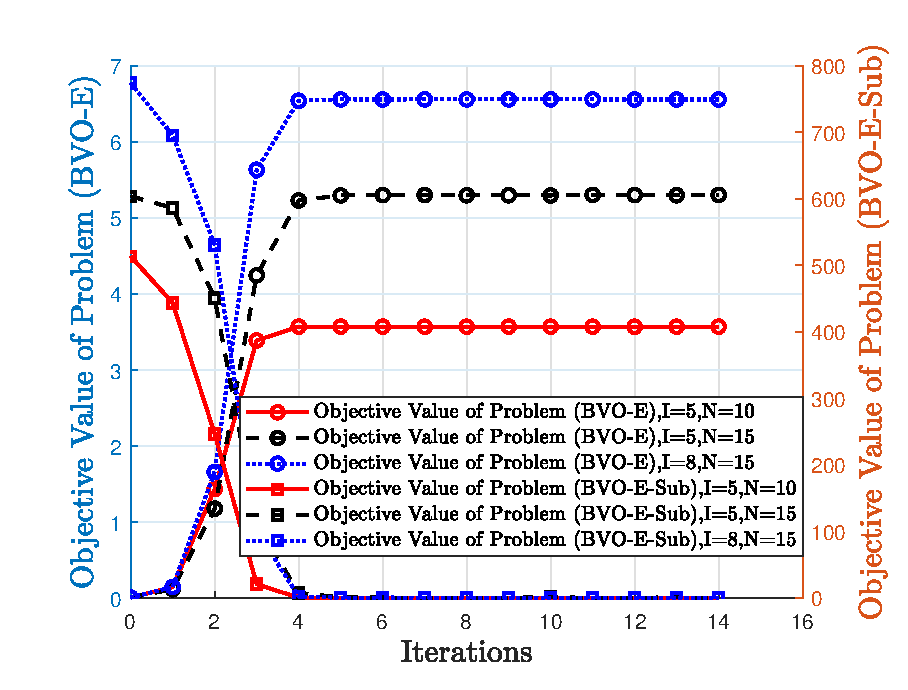
\includegraphics[width=0.6\textwidth]{figs_twc1_cld/Figure3a.eps}\label{3a}}
	\subfigure[Convergence of Algorithm 2] {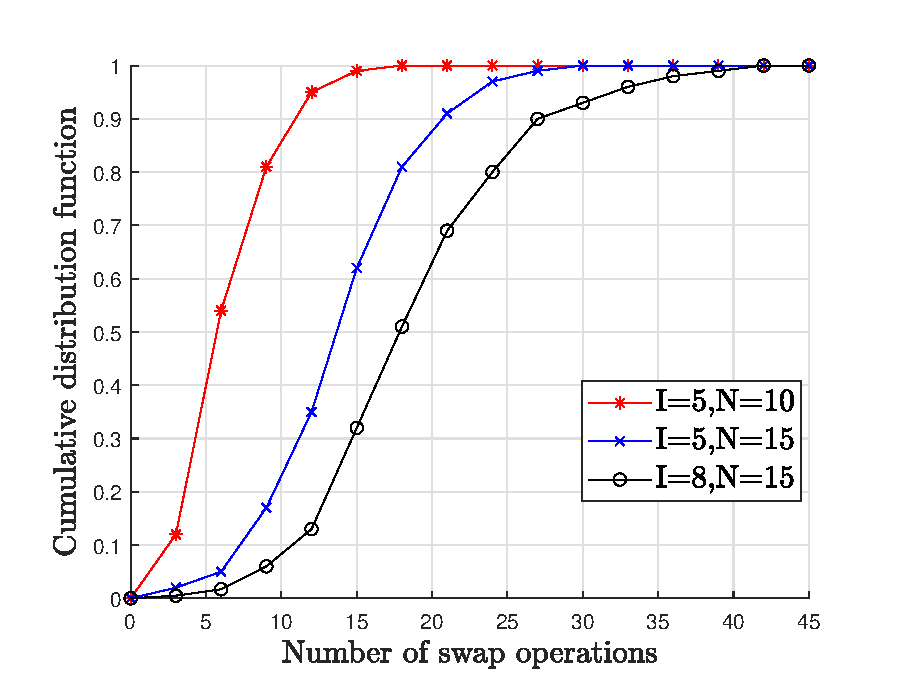
\includegraphics[width=0.6\textwidth]{figs_twc1_cld/Figure3b.eps}\label{3b}}
	\subfigure[Snapshot under $I=5$, $N=10$] {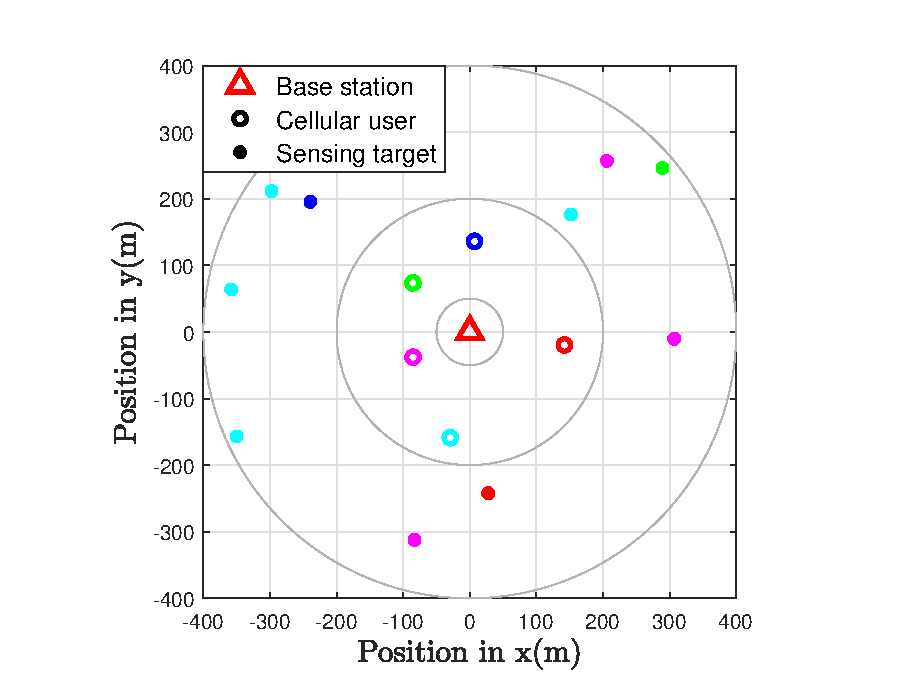
\includegraphics[width=0.6\textwidth]{figs_twc1_cld/Figure3c.eps}\label{3c}}
	\caption{Convergence of proposed algorithms and snapshot of the final channel sharing overcomes}
	\label{fig:3}
\end{figure*}

Figure \ref{fig:3} validates the convergence and effectiveness of our Algorithm 1 and Algorithm 2 under three scenarios. Specifically, Figure \ref{3a} shows that the objective value of Problem (BVO-E) can converge rapidly for all the tested scenarios. Meanwhile, the objective value of Problem (BVO-E-Sub) converges almost to zero, which is consistent with the Dinkelbach's method. In Figure \ref{3b}, we perform extensive simulations and plot the cumulative distribution function of the number of swap operations for the matching game. Figure \ref{3b} demonstrates that Algorithm 2 can converge within a small number of iterations for all three scenarios. In the scenario with $I = 8, N = 15$, 45 swap operations on average are required to ensure the convergence of Algorithm 2. Furthermore, Figure \ref{3b} also indicates that an increase in the number of the CUs or STs leads to an increase in the number of swap operations, since there will be more available swap-blocking pairs. As a concrete example, Figure \ref{3c} shows a snapshot of the optimal channel sharing solution for the scenario with $I = 5, N = 10$ by using our Algorithm 3, where the CUs and STs with the same color mean that they use the same channel.
	


\begin{figure*}
	\centering
	\subfigure[With different numbers of the STs] {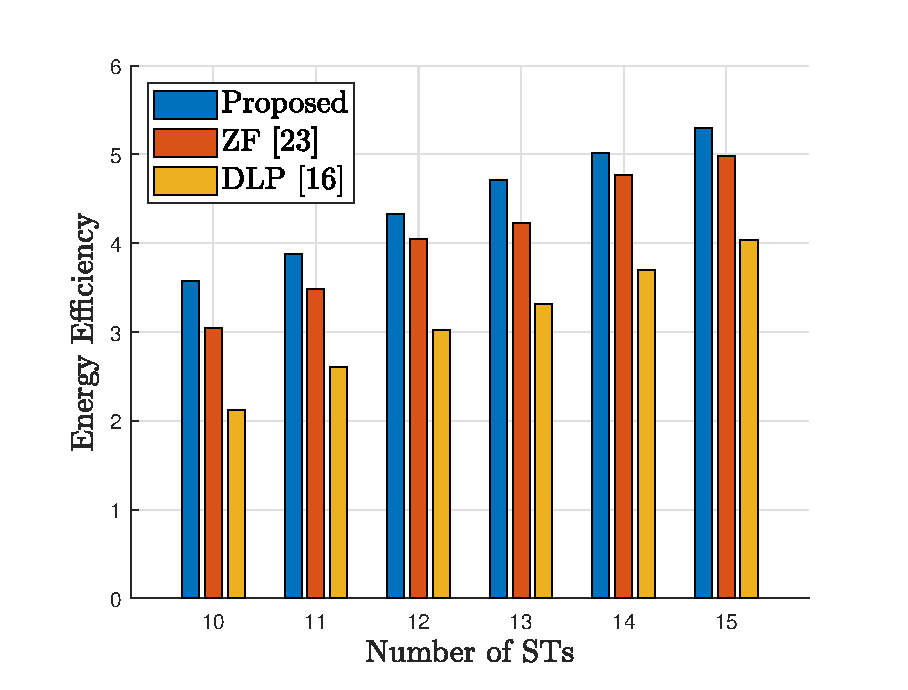
\includegraphics[width=0.6\textwidth]{figs_twc1_cld/Figure4a.eps}\label{4a}}
	\subfigure[With different numbers of the CUs] {\includegraphics[width=0.6\textwidth]{figs_twc1_cld/Figure4b.eps}\label{4b}}
	\subfigure[With different values of $\{J_i^{\text{max}}\}_{i\in\mathcal{I}}$] {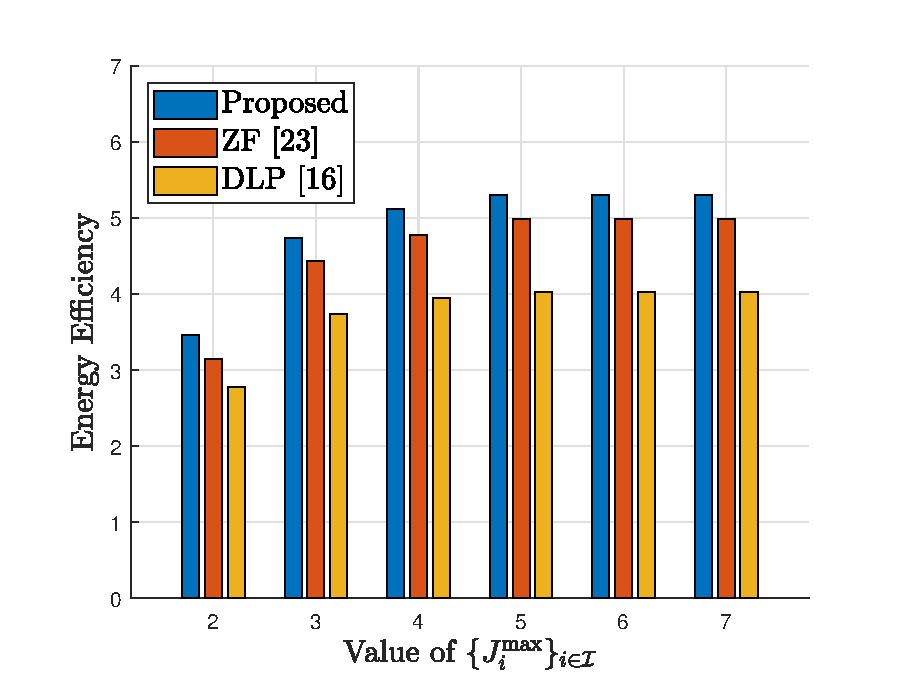
\includegraphics[width=0.6\textwidth]{figs_twc1_cld/Figure4c.eps}\label{4c}}
	\caption{Performance advantage of Algorithm 1}
	\label{fig:4}
\end{figure*}



Figure \ref{fig:4} demonstrates the performance of our proposed Algorithm 1 for solving Problem (MEE-BVO). Specifically, we use the zero-forcing (ZF) method \cite{twc1.9124713} and the double-layer penalty (DLP) method \cite{tvt.wang2022noma} as the comparison benchmarks. Figure \ref{fig:4} demonstrates that our Algorithm 1 outperforms the two benchmark algorithms in terms of improving energy efficiency. Figure \ref{4a} shows that the energy efficiency increases when the number of the STs increases, which is due to the increase in the total REIR. Figure \ref{4b} shows that the energy efficiency increases as the number of the CUs increases, which is due to the reduction of mutual interference among STs. Figure \ref{4c} shows that as the maximum number of the STs which can be sensed by each CU's channel increases, the energy efficiency gradually increases until all STs are sensed by their respective most preferred CUs' channels.


\begin{figure*}
	\centering
	\subfigure[With different numbers of the STs] {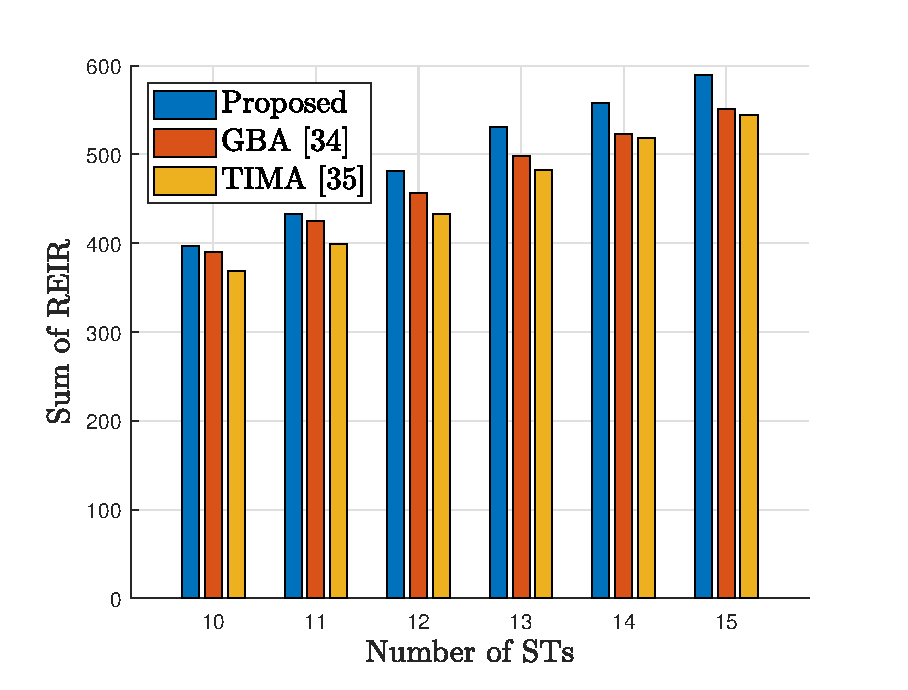
\includegraphics[width=0.6\textwidth]{figs_twc1_cld/Figure5a.eps}\label{5a}}
	\subfigure[With different numbers of the CUs] {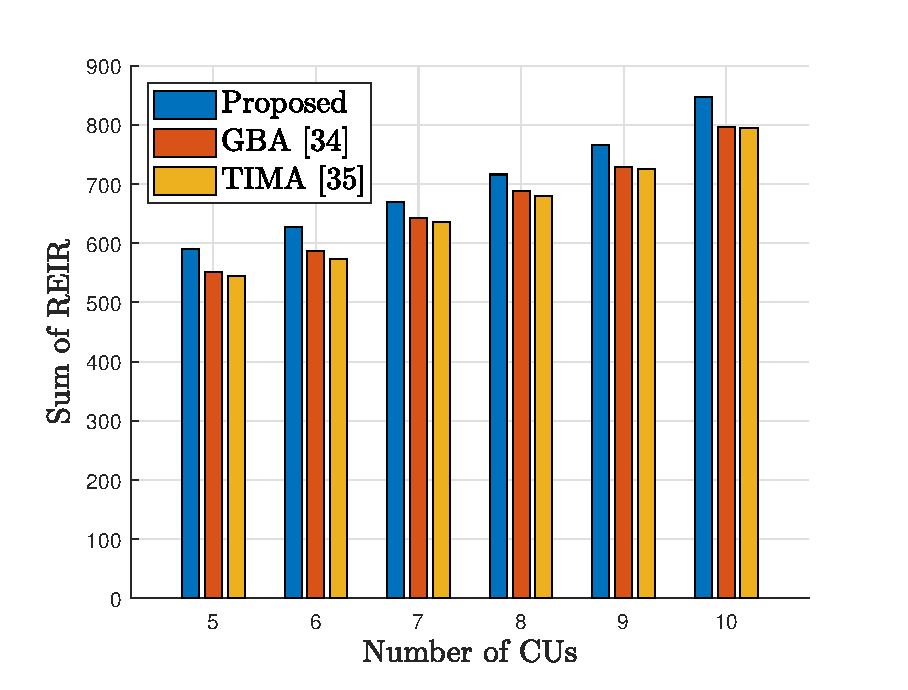
\includegraphics[width=0.6\textwidth]{figs_twc1_cld/Figure5b.eps}\label{5b}}
	\subfigure[With different values of $\{J_i^{\text{max}}\}_{i\in\mathcal{I}}$] {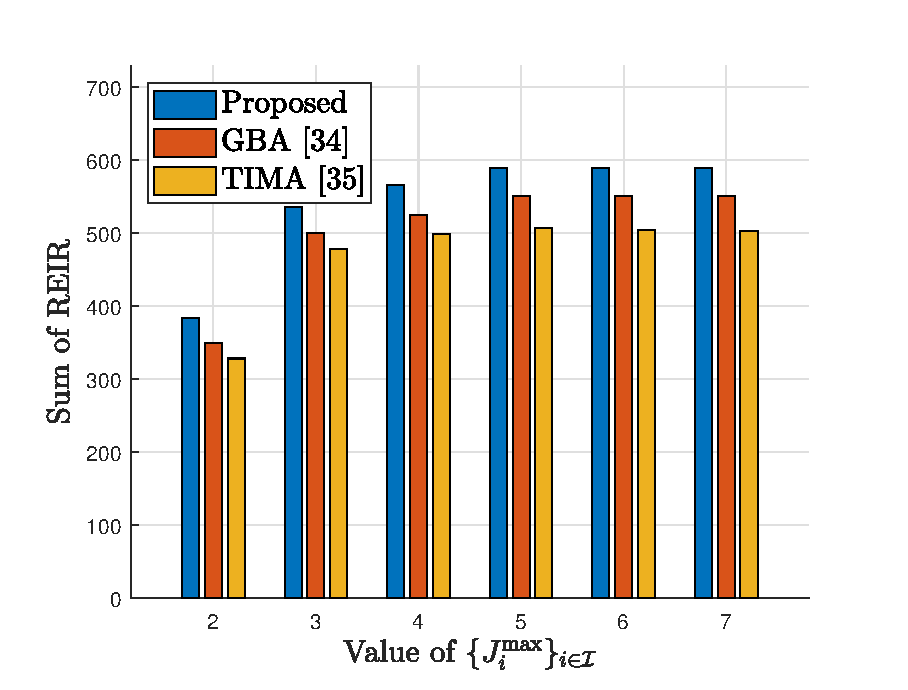
\includegraphics[width=0.6\textwidth]{figs_twc1_cld/Figure5c.eps}\label{5c}}
	\caption{Performance advantage of Algorithm 2}
	\label{fig:5}
\end{figure*}

Figure \ref{fig:5} demonstrates the performance of our proposed Algorithm 2 for solving Problem (MEE-SSO). We use the following two approaches as the comparison benchmarks, i.e., 1) greedy-based allocation (GBA) method based on mutual interference among STs \cite{twc1.7308022} and 2) the total interference minimization allocation (TIMA) method which aims at minimizing $\sum_{n\in\mathcal{N}}\sum_{i\in\mathcal{I}}x_{ni}\mathbf{Tr}\left(\mathbf{H}_i\mathbf{V}_n\right)$ \cite{twc1.7087396}. Figure \ref{fig:5} demonstrates that our Algorithm 2 outperforms the two benchmark algorithms in terms of improving the sum of REIR. Figure \ref{5a} shows that the sum of REIR increases as the number of the STs increases. Figure \ref{5b} shows that the sum of REIR increases as the number of the CUs increases. Figure \ref{5c} again demonstrates the advantage of our Algorithm 2 under different values of $J_i^{\text{max}}$, i.e., the maximum number of the STs which can be sensed by each CU's channel.


\begin{figure*}
	\centering
	\subfigure[Comparison of accuracy] {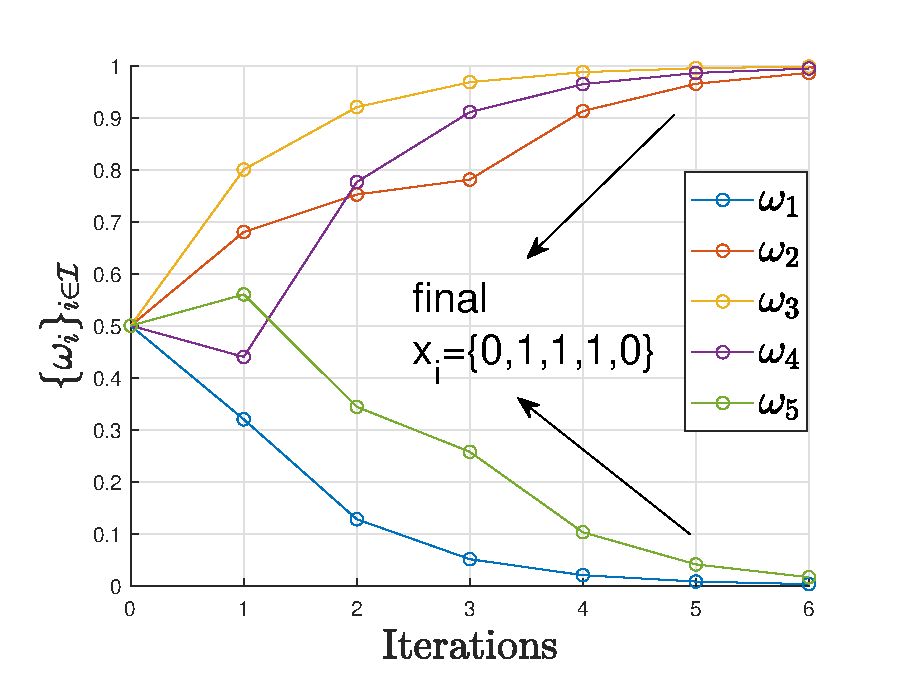
\includegraphics[width=0.6\textwidth]{figs_twc1_cld/Figure6a.eps}\label{6a}}
	\subfigure[Comparison of accuracy] {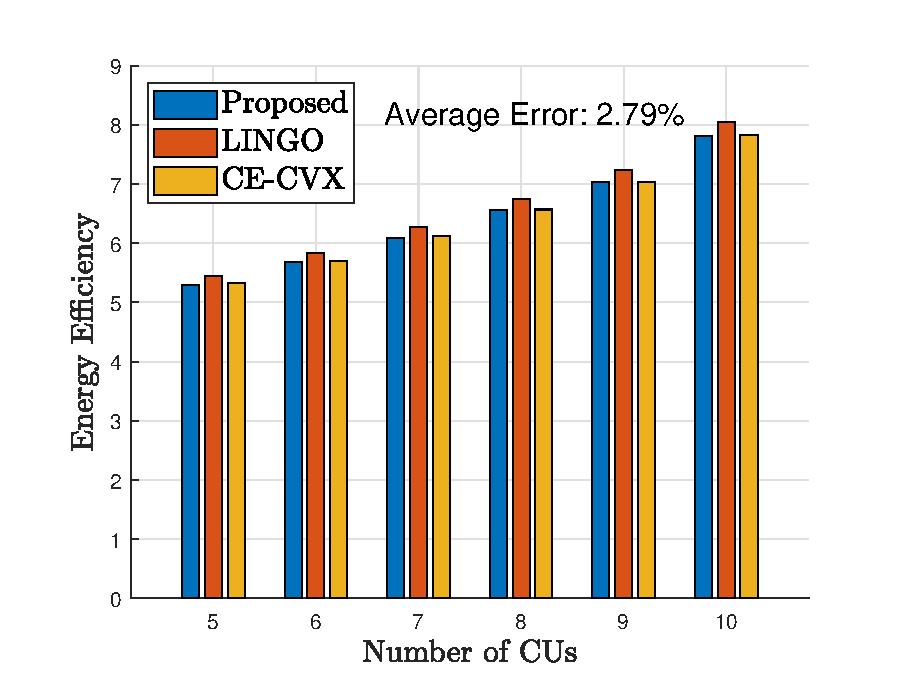
\includegraphics[width=0.6\textwidth]{figs_twc1_cld/Figure6b.eps}\label{6b}}
	\subfigure[Comparison of efficiency] {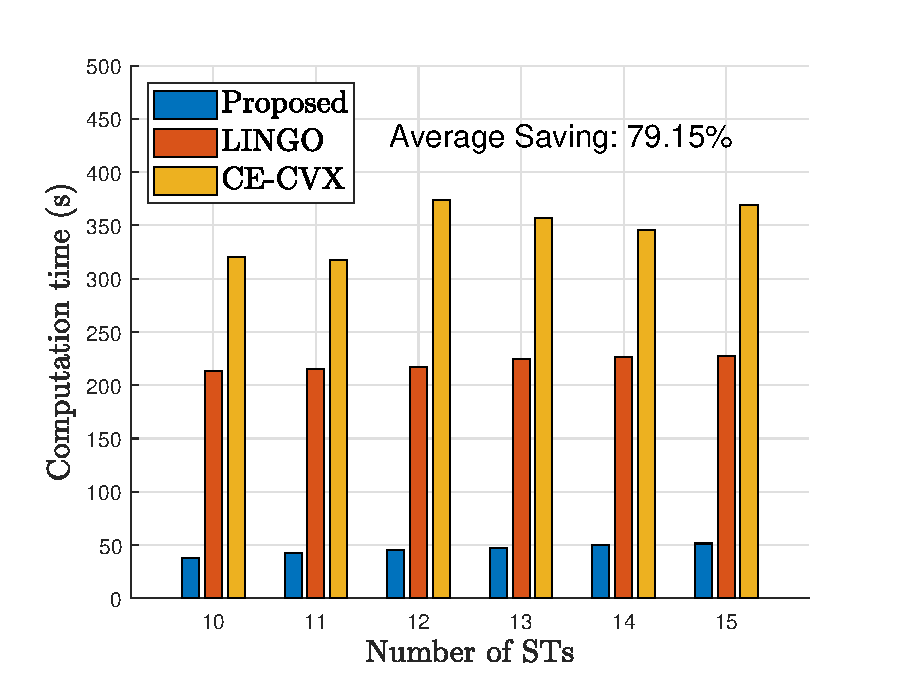
\includegraphics[width=0.6\textwidth]{figs_twc1_cld/Figure6c.eps}\label{6c}}
	\caption{Accuracy and efficiency of Algorithm 3}
	\label{fig:6}
\end{figure*}

	
Figure \ref{fig:6} validates the accuracy and efficiency of Algorithm 3. Specifically, since our proposed alternating optimization method cannot guarantee to achieve the optimal solution of the original problem, we compare the results with the solution of LINGO \cite{twc1.schrage2006optimization}. In addition, we compare it with the scheme of learning which solves Problem (MEE-SSO) with the cross-entropy (CE) algorithm \cite{twc1.de2005tutorial} and solves Problem (MEE-BVO) with CVX (which is a solver for convex optimizations), denoted by CE-CVX in Figure \ref{fig:6}. Figures \ref{6a} and \ref{6b} show the accuracy of our Algorithm 3. Specifically, the results in Figure \ref{6a} and Figure \ref{6b} demonstrate that our algorithm can outperform the CE-CVX scheme while achieving the close-to-optimal solution compared to LINGO. For the sake of clear illustration, we also mark the average error between our proposed algorithm and the result of LINGO on the top of the two subplots, with the maximum average error no greater than 3\%, which is acceptable. Furthermore, Figure \ref{6c} shows the computation efficiency of our Algorithm 3. The results show that our algorithm can significantly reduce the computation time compared to the other two benchmark schemes, i.e., LINGO and CE-CVX.



\begin{figure}
	\centering
	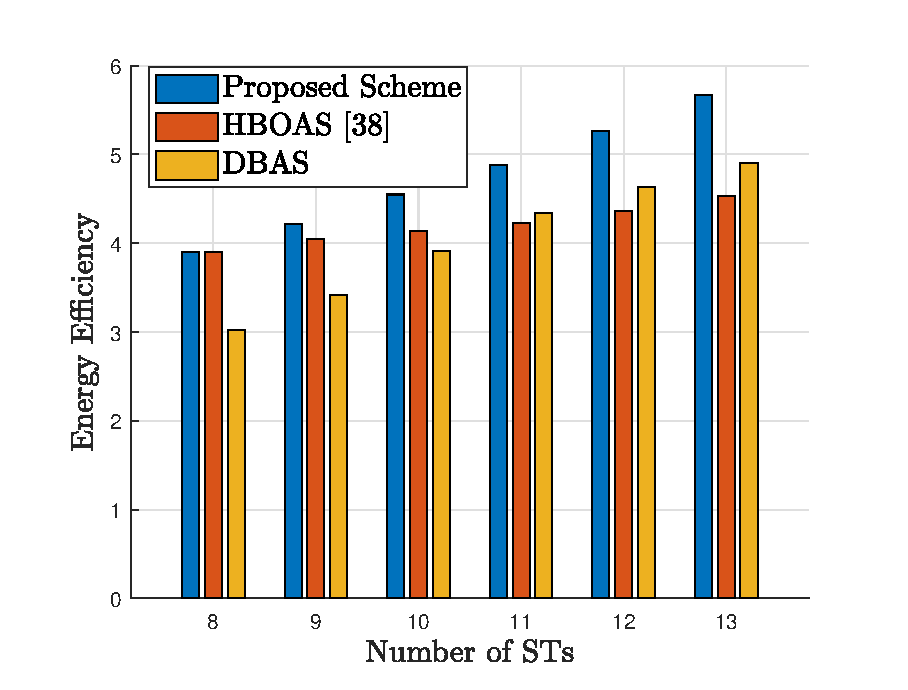
\includegraphics[width=0.6\textwidth]{figs_twc1_cld/Figure7.eps}
	\caption{Performance advantage of our channel sharing aided ISAC}
	\label{fig:7}
\end{figure}


Figure \ref{fig:7} demonstrates the performance advantage of proposed channel sharing aided ISAC under the setting of $I=8$. We use the following two schemes as the comparison benchmarks, i.e., 1) Hungarian-based orthogonal allocation scheme (HBOAS) which allocates the channels to the STs orthogonally (i.e., $\{J_i^{\text{max}}\}_{i\in\mathcal{I}}=1$) \cite{twc1.feng2013device} and 2) distance-based allocation scheme (DBAS) enables the STs closest to CU $i$ to share CU $i$'s channel. Figure \ref{fig:7} validates that our proposed channel sharing scheme can outperform the other two benchmark schemes.

\section{Conclusion} \label{chap2_sec_conclusion}

In this chapter, we have investigated an energy-efficient channel sharing aided ISAC with sensing scheduling. 
Specifically, the ISAC BS performs the multi-target sensing by reusing the CUs' channels while guaranteeing each individual CU's throughput requirement. 
We have proposed a joint optimization of multi-target sensing scheduling, the BS's transmitting beamforming vectors, and its receiving beamforming vectors for the STs, with the objective of maximizing the energy efficiency for radar sensing.
Despite that the formulated joint optimization problem is strictly non-convex, we have exploited a framework of alternating optimization and proposed the corresponding algorithms for solving the problem. Specifically, we have utilized Dinkelbach's method and Lagrange duality to obtain the beamforming vectors, and formulated the sensing scheduling problem as a matching game.
Numerical results have been provided to validate the effectiveness of our algorithms and the performance advantages of the proposed channel sharing aided ISAC. 




